\documentclass[a4paper,11pt]{article}
\usepackage[utf8]{inputenc}
\usepackage[T1]{fontenc}
\usepackage{lmodern}
\usepackage[margin=2.5cm]{geometry}
\usepackage{graphicx}
\usepackage{booktabs}
\usepackage{array}
\usepackage{float}
\usepackage{enumitem}

\title{Trabalho Prático 1 --- Segmentação de Embalagens de Produtos Avícolas}
\author{Bruno Silveira}
\date{}

\begin{document}
\maketitle

\section{Introdução}

Este relatório documenta a primeira etapa do projeto de Processamento Digital de Imagens (PDI)
aplicado a embalagens de produtos avícolas. O objetivo desta etapa é localizar e segmentar
automaticamente, em imagens capturadas em ambiente industrial (esteira com câmera fixa), a
região da embalagem que contém o nome do produto --- sem realizar classificação ou
reconhecimento de texto, que é o escopo da segunda etapa do projeto (T2).

O conjunto de dados contém 18 classes de produto, distribuídas em dois tipos de embalagem física
(bandeja e selada), com cerca de 50 imagens por classe. As imagens apresentam desafios típicos de
ambiente industrial: reflexos, deformação da embalagem, variação de iluminação e de
posicionamento/orientação do produto.

\section{Objetivos}

\begin{itemize}[nosep]
  \item Desenvolver um pipeline de segmentação que localize a região do rótulo com o nome do
        produto em cada imagem, usando exclusivamente técnicas clássicas de PDI (espaços de cor,
        limiarização, operações morfológicas, filtragem espacial, transformações geométricas),
        sem bibliotecas de segmentação baseadas em IA.
  \item Tratar os dois layouts físicos de embalagem do dataset --- bandeja e selado --- cada um
        com um pipeline próprio, já que a posição e a forma do rótulo diferem entre eles.
  \item Minimizar falsos positivos (recorte gerado sem o nome do produto, ou com texto
        irrelevante), mesmo que isso implique deixar de gerar recorte em alguns casos --- o
        enunciado trata falso positivo como erro mais grave que detecção perdida.
  \item Garantir que o pipeline rode fim a fim sobre um conjunto de imagens novo sem nenhuma
        alteração de código, já que uma parte da avaliação usa imagens inéditas no dia da
        apresentação.
\end{itemize}

\section{Desenvolvimento}

Ambos os pipelines seguem a mesma estrutura: uma sequência linear de etapas, cada uma uma função
pura que opera sobre a saída da etapa anterior, com todos os parâmetros centralizados em um
dicionário de configuração único em vez de espalhados como literais no código --- o que permite
recalibrar o pipeline inteiro sem editar a lógica.

\subsection{Pipeline bandeja (\texttt{segmentador\_colab.ipynb})}

O rótulo, nesse tipo de embalagem, aparece como uma região destacada mas não fixa dentro do
quadro, exigindo detecção por contorno:

\begin{enumerate}[nosep]
  \item \textbf{Extração de brilho}: conversão BGR→LAB e equalização adaptativa de histograma
        (CLAHE) no canal L, para compensar iluminação industrial desigual.
  \item \textbf{Suavização}: filtro de mediana, para remoção de ruído sem borrar bordas de texto.
  \item \textbf{Binarização}: limiarização de Otsu com deslocamento manual
        (\texttt{thresh\_offset}) --- Otsu sozinho tende a escolher um limiar entre o texto
        escuro do rótulo e o fundo mais claro, então é ajustado empiricamente.
  \item \textbf{Aplicação de ROI}: zera uma margem fixa de borda, removendo esteira e paredes
        laterais do quadro de detecção.
  \item \textbf{Morfologia}: fechamento (junta o texto do rótulo em um único blob) seguido de
        abertura (remove blobs de ruído pequenos).
  \item \textbf{Classificação de regiões}: extração de contornos com filtros geométricos (área,
        proporção largura/altura, altura mínima, solidez), registrando o motivo de rejeição de
        cada região descartada para facilitar depuração.
  \item \textbf{Supressão de sobreposição (NMS)}: supressão por IoU entre caixas candidatas;
        apenas a maior caixa aceita é mantida.
  \item \textbf{Recorte quadrado}: recorte centralizado na caixa vencedora (lado =
        max(largura, altura)), sem redimensionamento.
\end{enumerate}

\subsection{Pipeline selado (\texttt{segmentador\_selado.ipynb})}

Nesse tipo de embalagem o rótulo ocupa uma faixa horizontal fixa, o que muda a estratégia de
detecção:

\begin{enumerate}[nosep]
  \item Alongamento de contraste por percentil.
  \item Recorte de ROI com máscara fixa sobre a região de FPS/timestamp sobreposta pela câmera.
  \item Morfologia top-hat, para realçar o texto escuro sobre fundo claro na faixa do rótulo.
  \item Limiarização adaptativa/fixa.
  \item Extração de componentes conectados, filtrados por área.
  \item \emph{Clustering} espacial dos componentes restantes, para reagrupar texto multi-letra em
        uma única região, preferindo o agrupamento de proporção larga (horizontal) --- que é a
        orientação do texto nesse tipo de embalagem.
\end{enumerate}

\section{Resultados}

A Figura~1 mostra um exemplo de resultado por classe (recortes gerados pelo pipeline), para as 7
classes de embalagem bandeja e as 11 classes de embalagem selada do dataset. A saída completa do
pipeline (todas as imagens, todas as classes) não é anexada a este relatório por volume; pode ser
regenerada rodando os notebooks sobre o dataset local.

\begin{figure}[H]
\centering
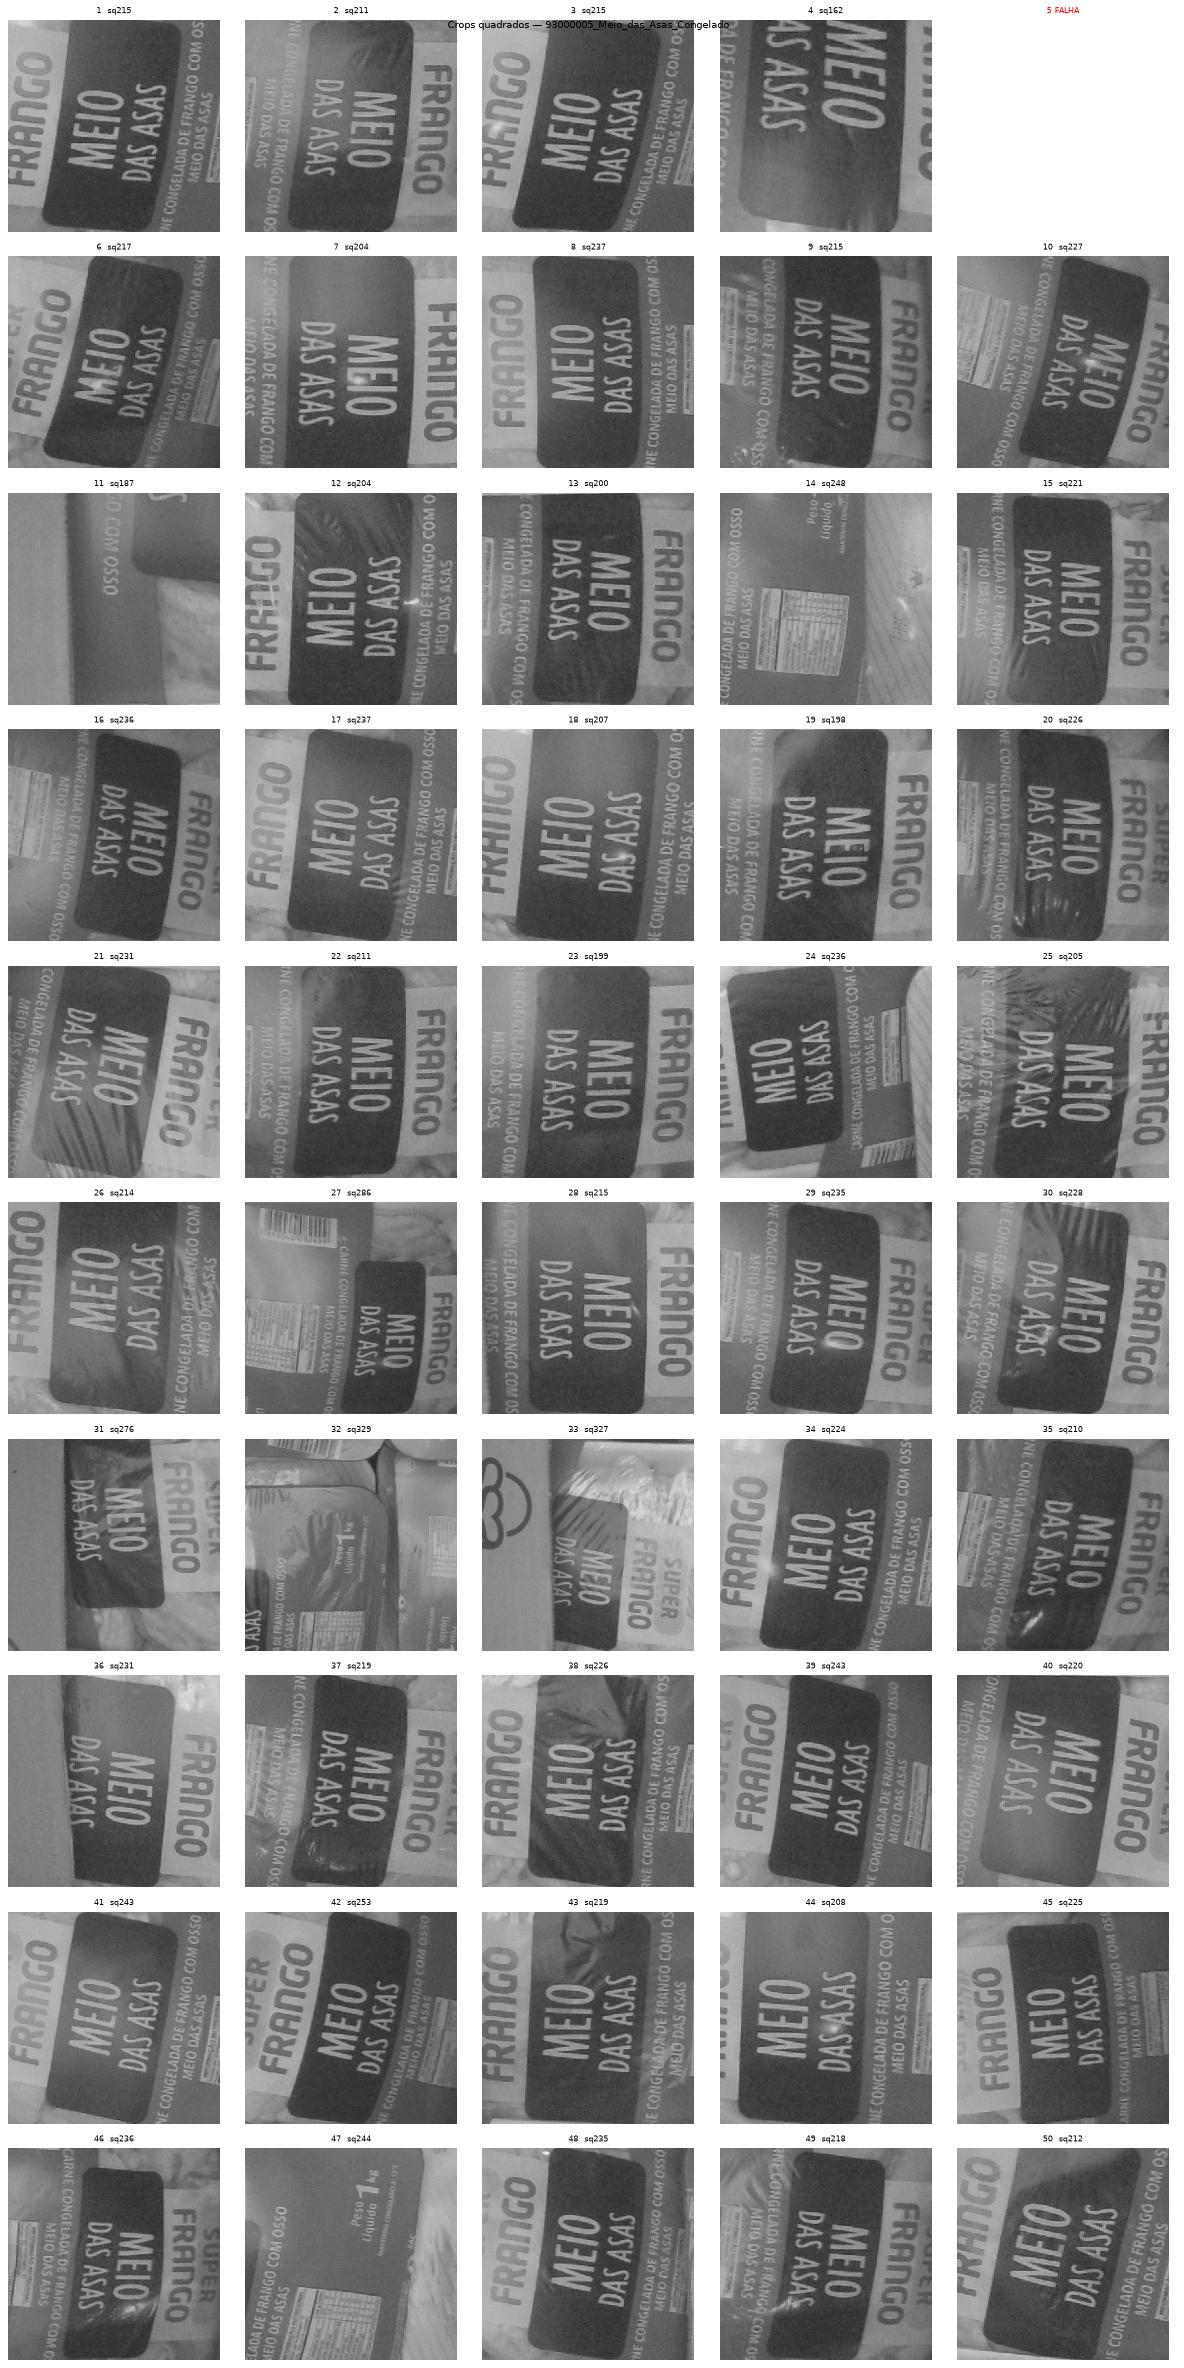
\includegraphics[width=0.85\textwidth]{resultados-exemplo/bandeja/93000005_Meio_das_Asas_Congelado_2_crops.png}
\caption{Meio das Asas Congelado (bandeja).}
\end{figure}

\begin{figure}[H]
\centering
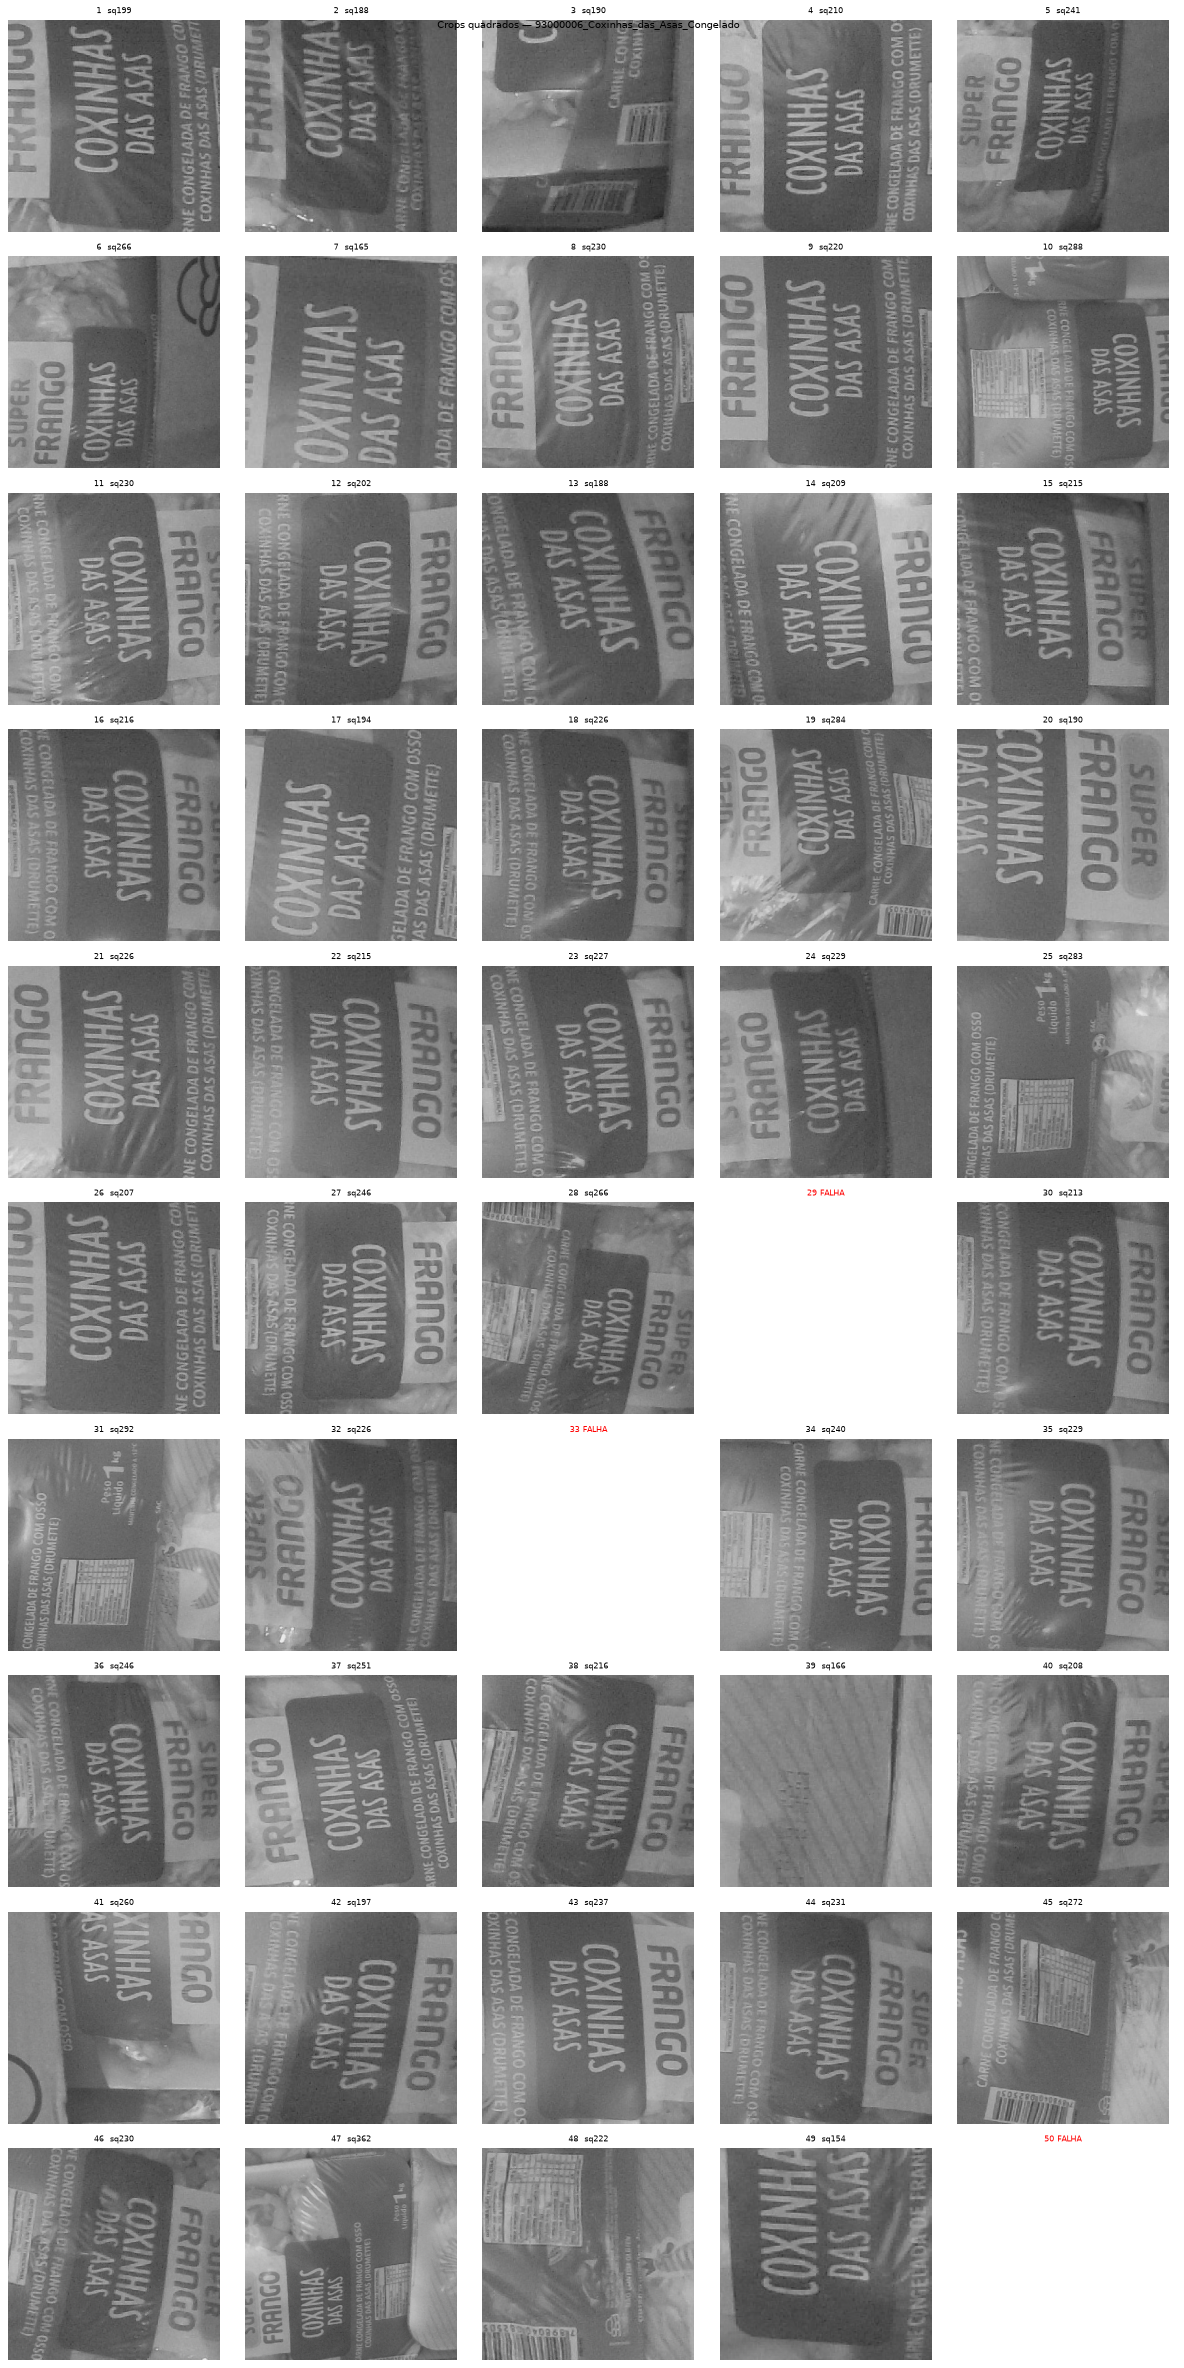
\includegraphics[width=0.85\textwidth]{resultados-exemplo/bandeja/93000006_Coxinhas_das_Asas_Congelado_2_crops.png}
\caption{Coxinhas das Asas Congelado (bandeja).}
\end{figure}

\begin{figure}[H]
\centering
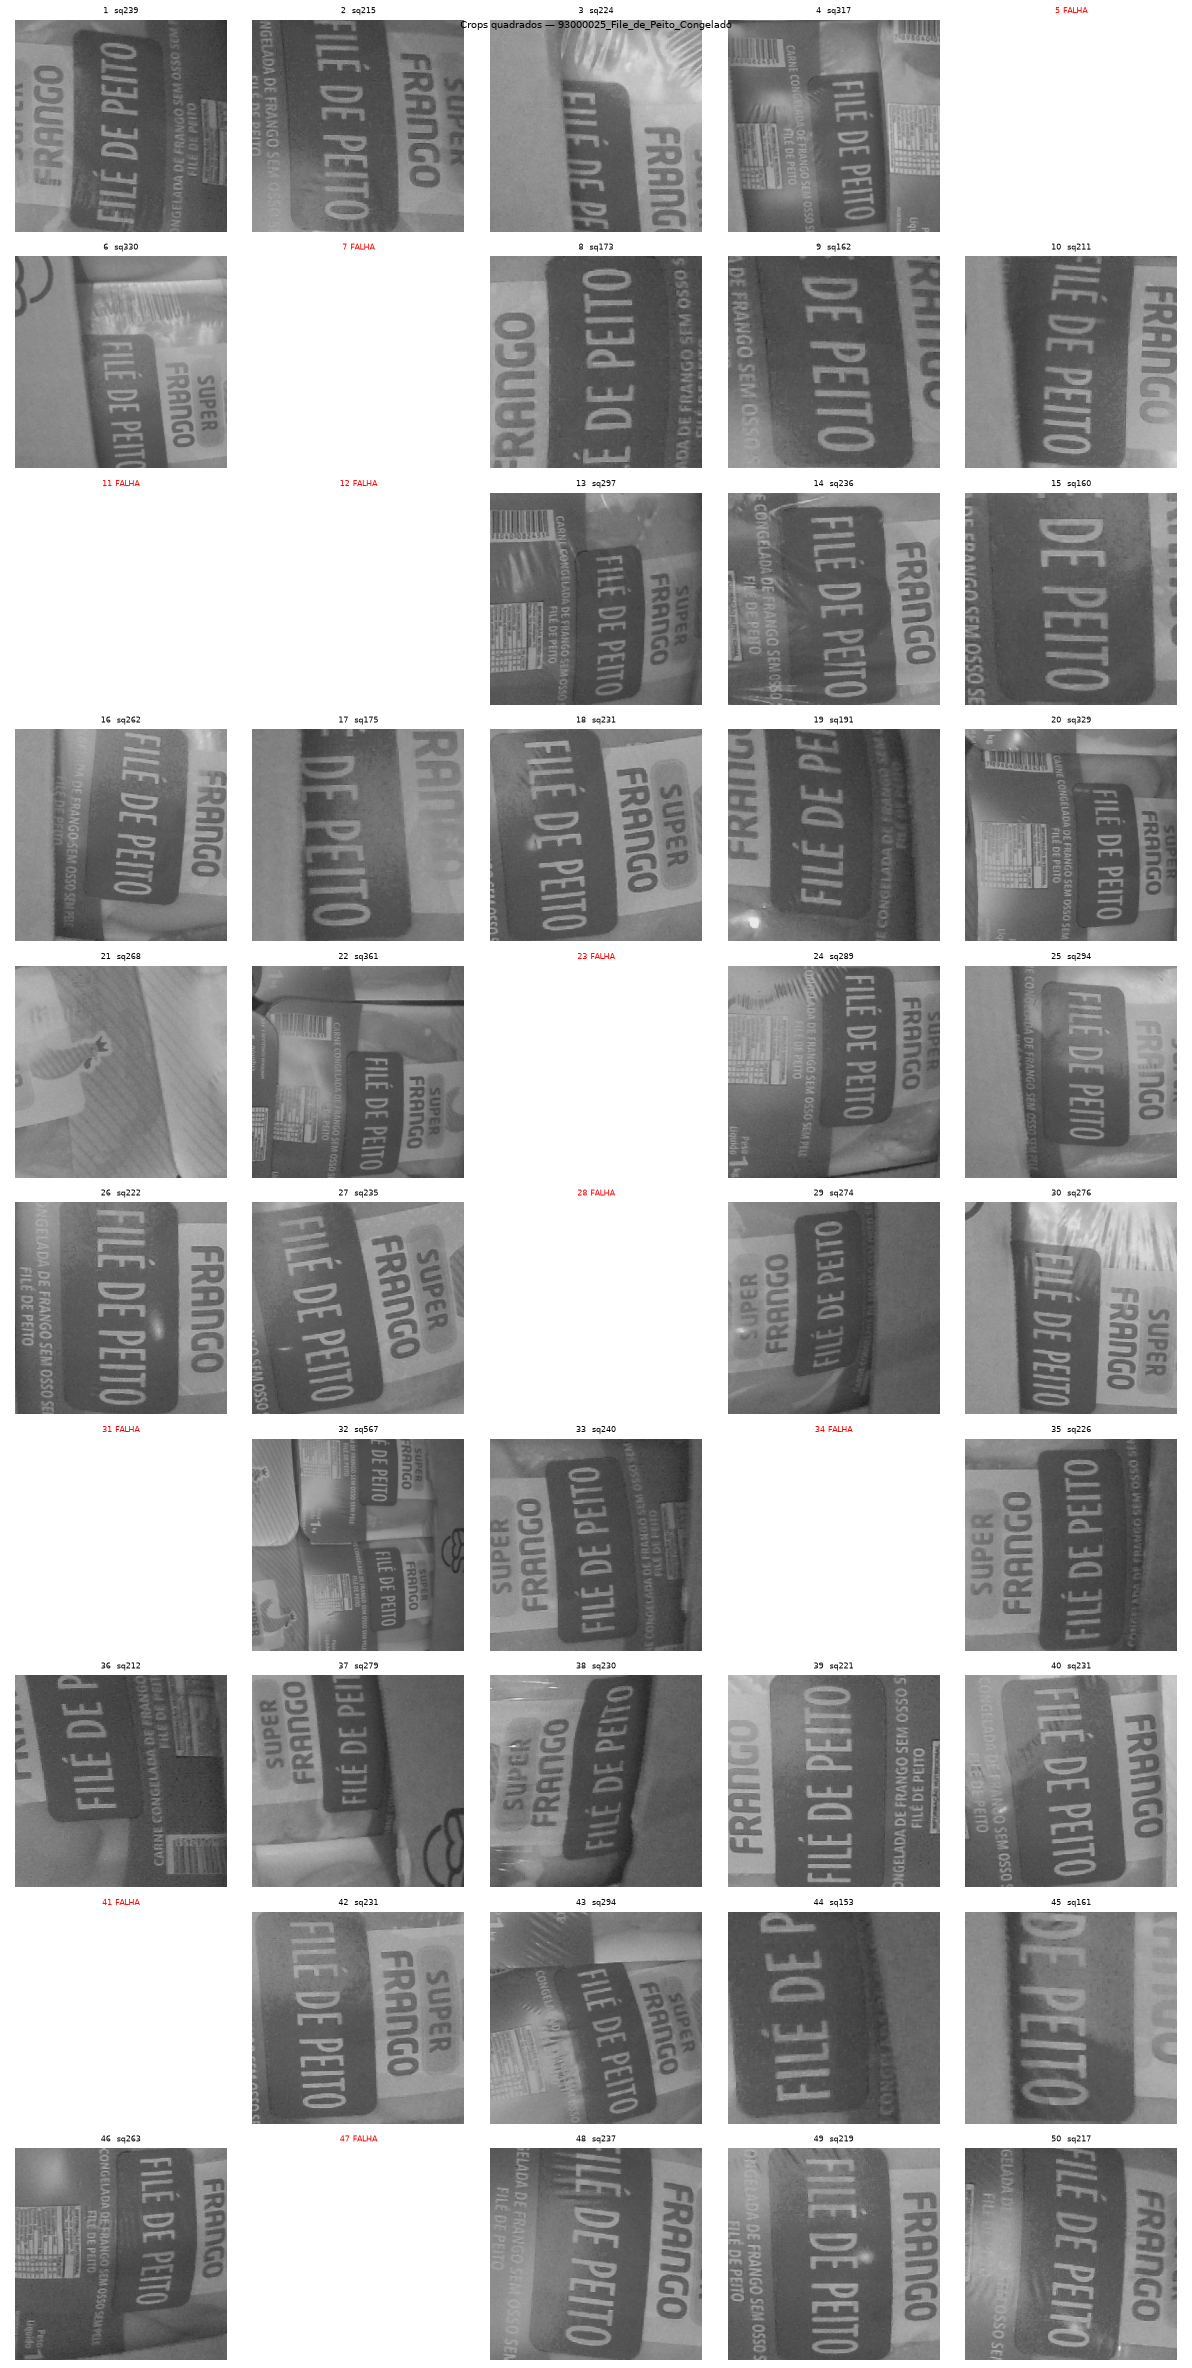
\includegraphics[width=0.85\textwidth]{resultados-exemplo/bandeja/93000025_File_de_Peito_Congelado_2_crops.png}
\caption{Filé de Peito Congelado (bandeja).}
\end{figure}

\begin{figure}[H]
\centering
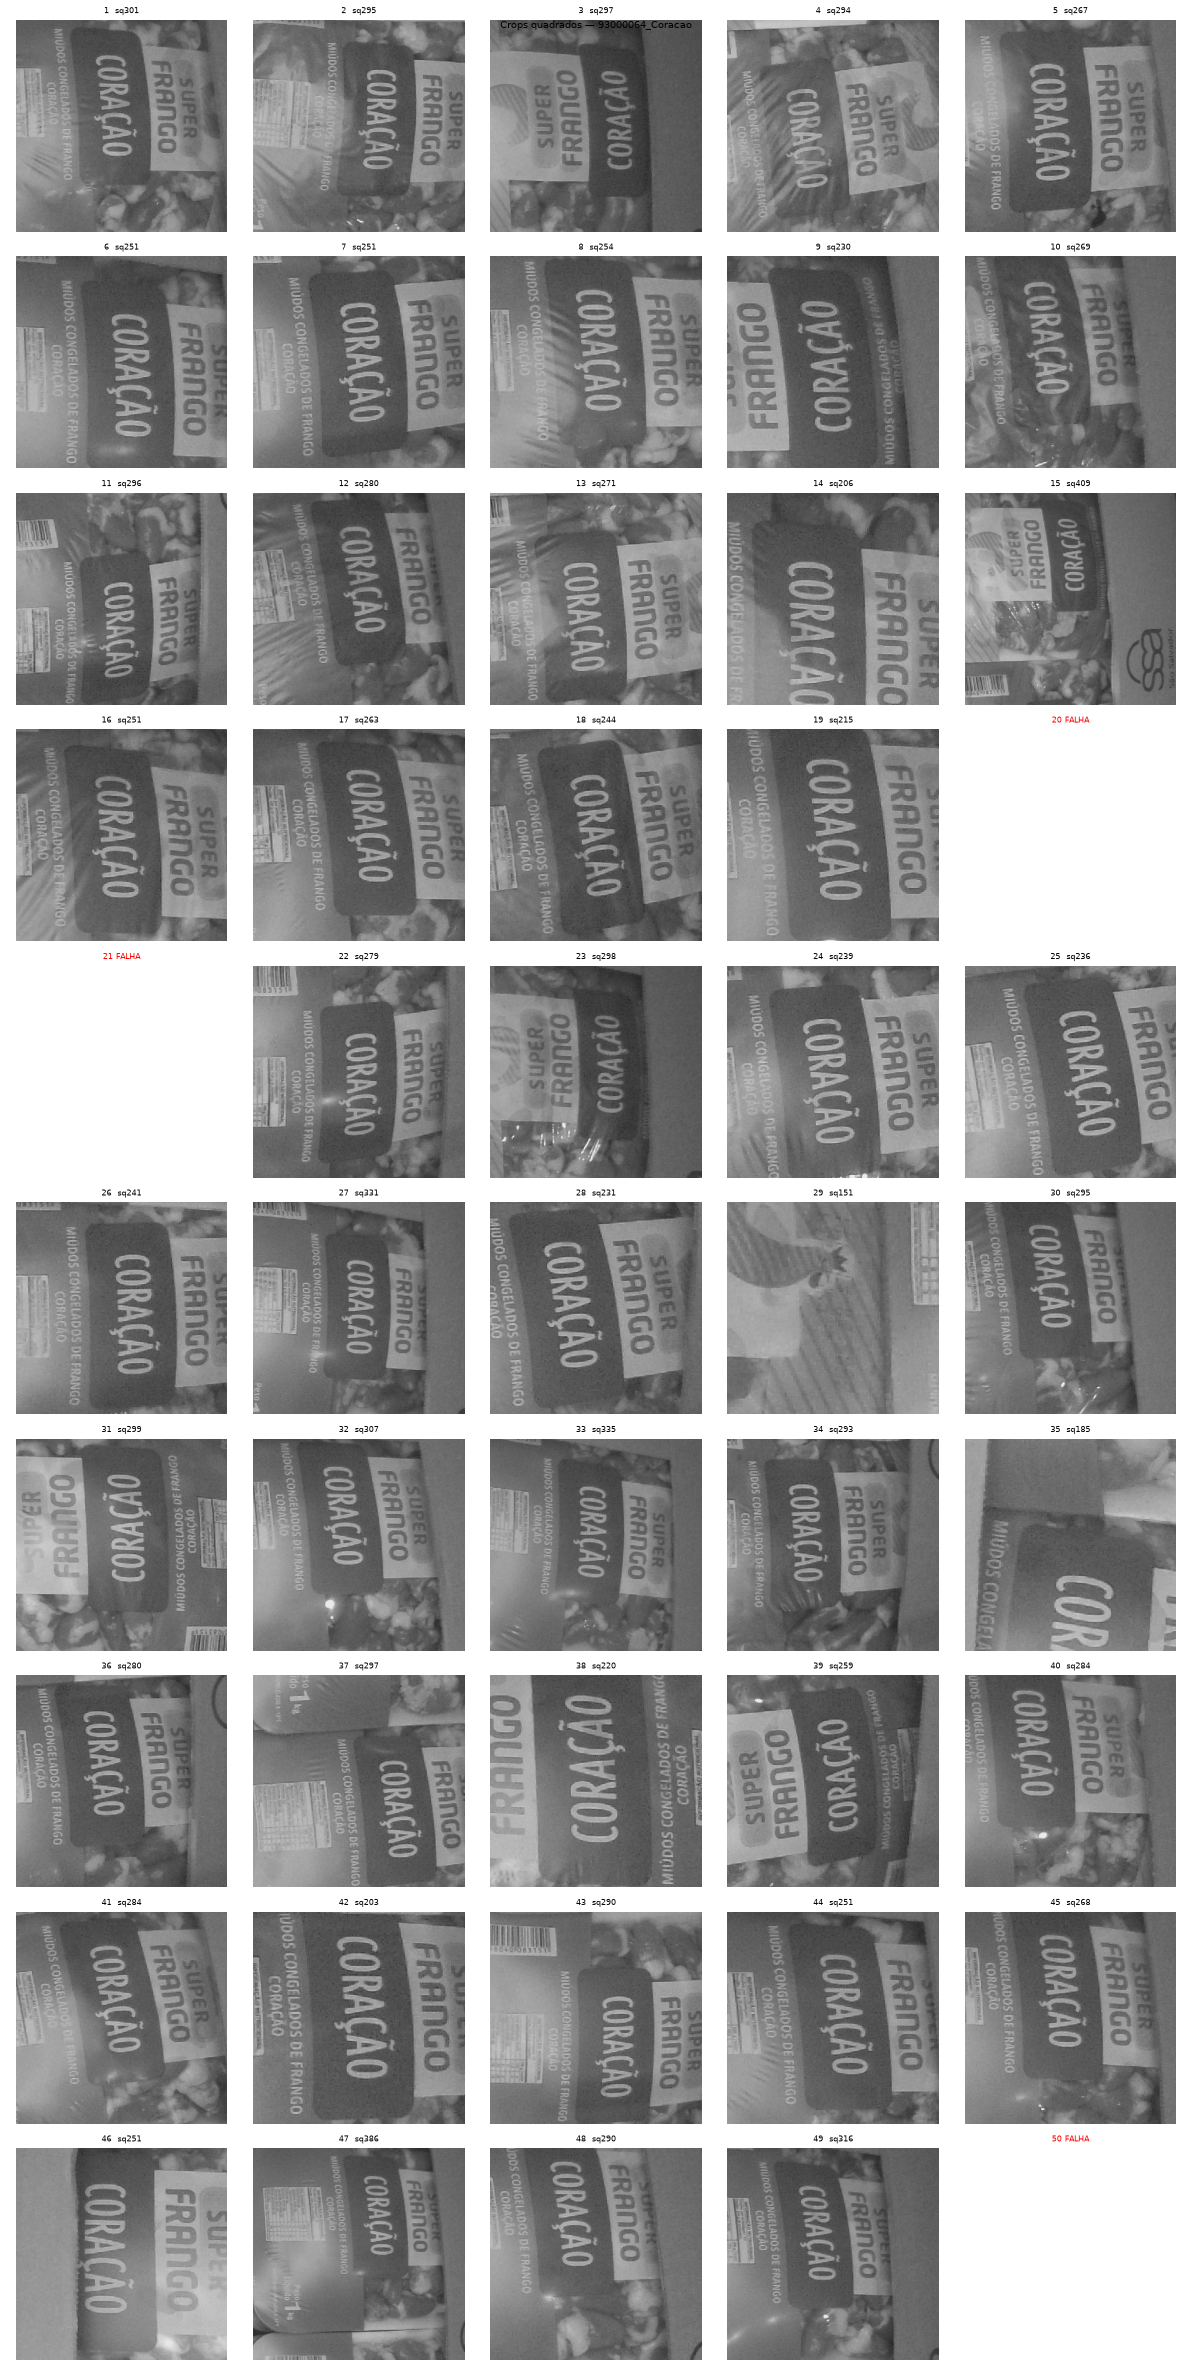
\includegraphics[width=0.85\textwidth]{resultados-exemplo/bandeja/93000064_Coracao_2_crops.png}
\caption{Coração (bandeja).}
\end{figure}

\begin{figure}[H]
\centering
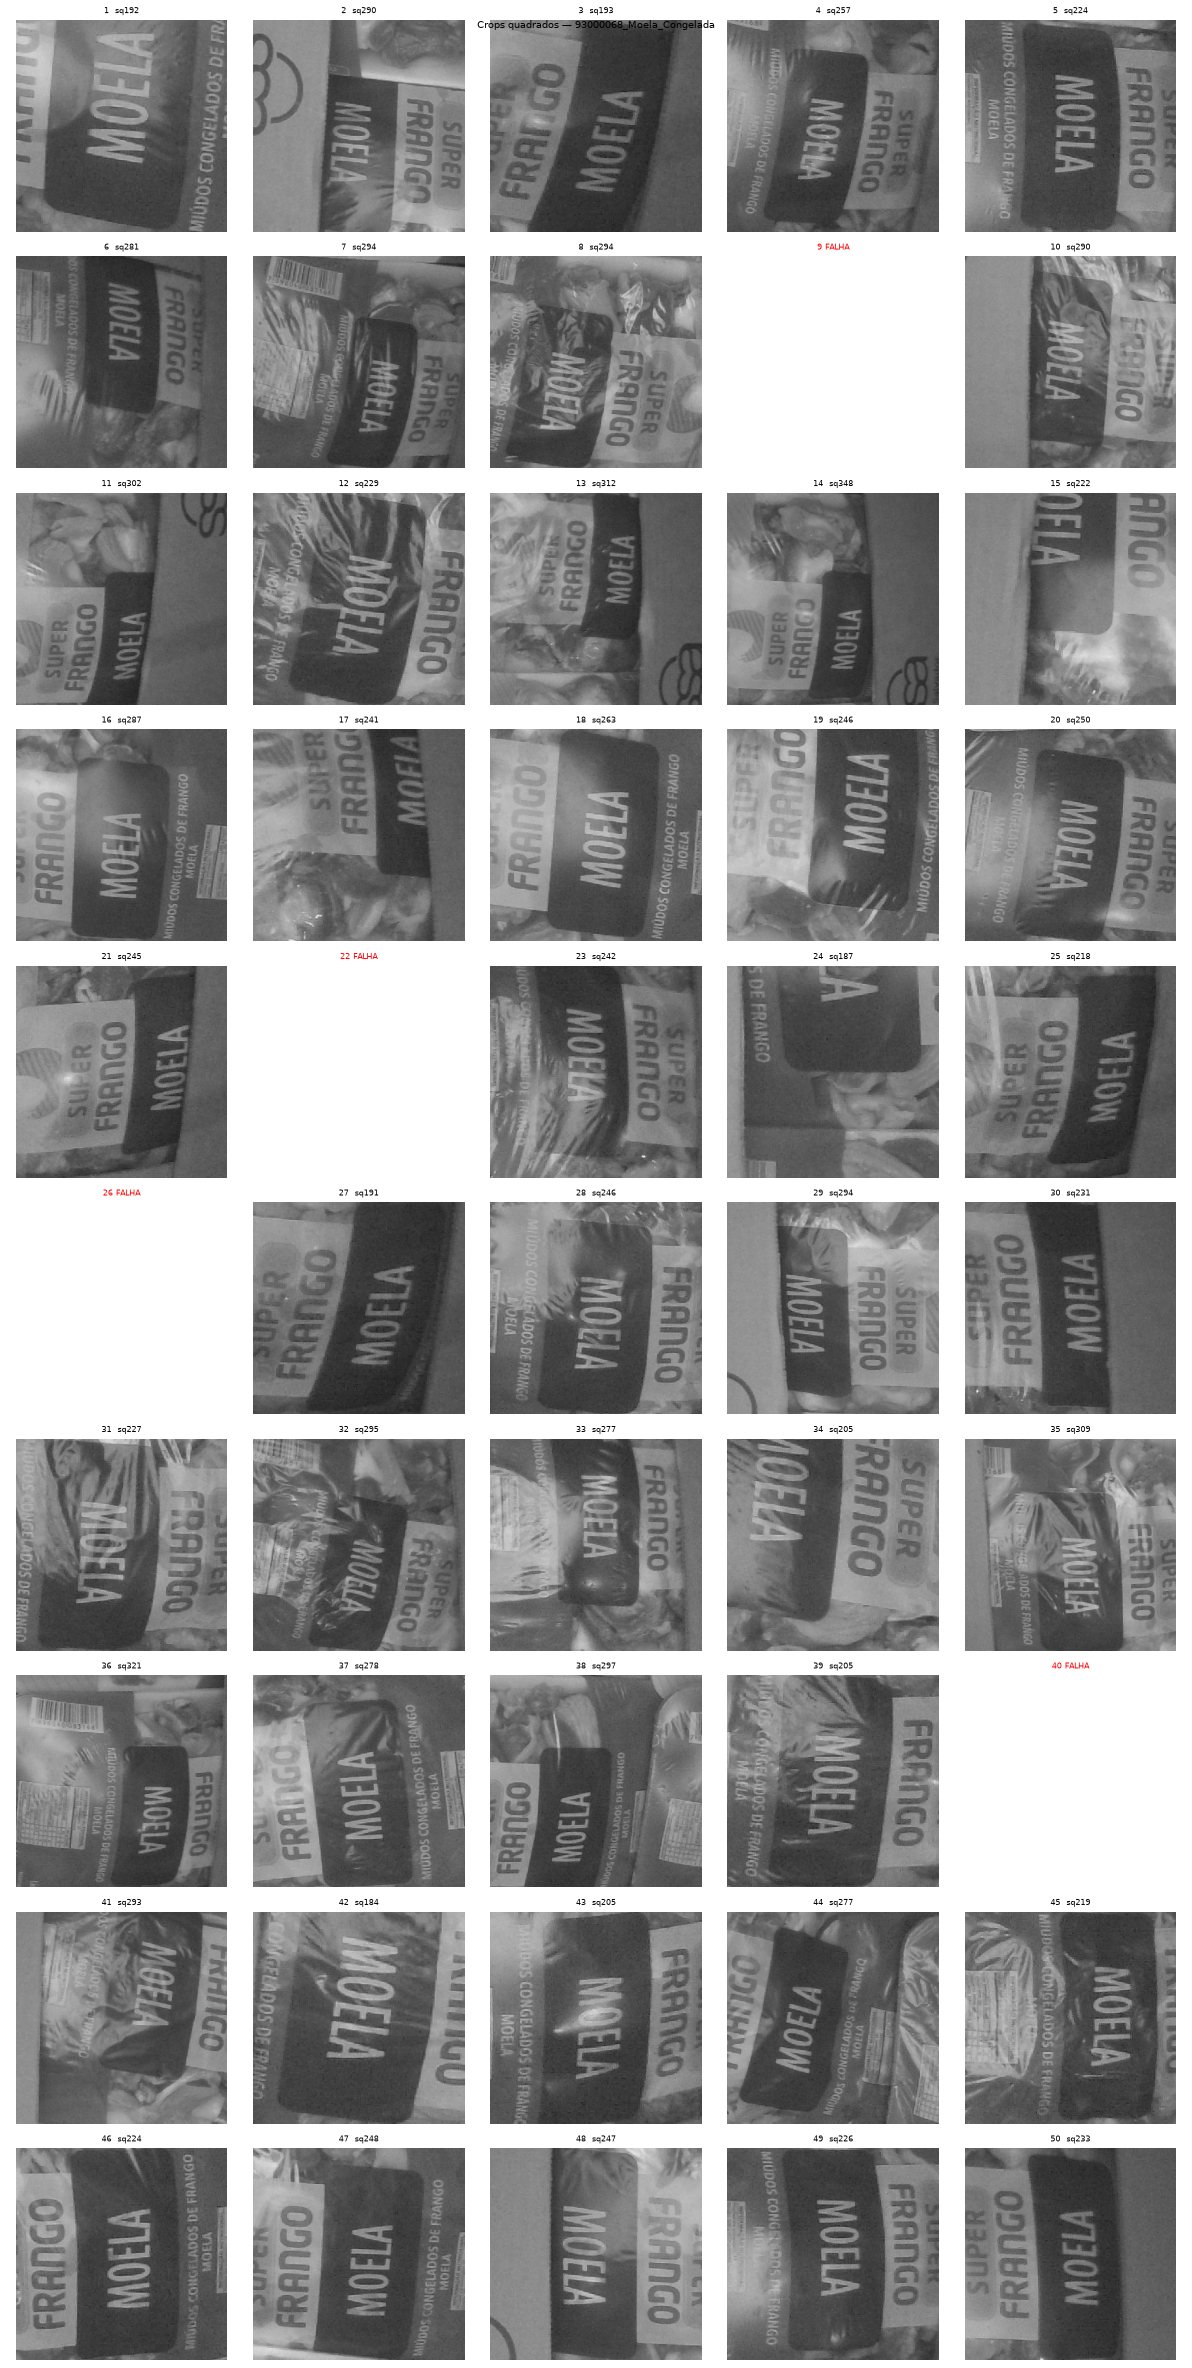
\includegraphics[width=0.85\textwidth]{resultados-exemplo/bandeja/93000068_Moela_Congelada_2_crops.png}
\caption{Moela Congelada (bandeja).}
\end{figure}

\begin{figure}[H]
\centering
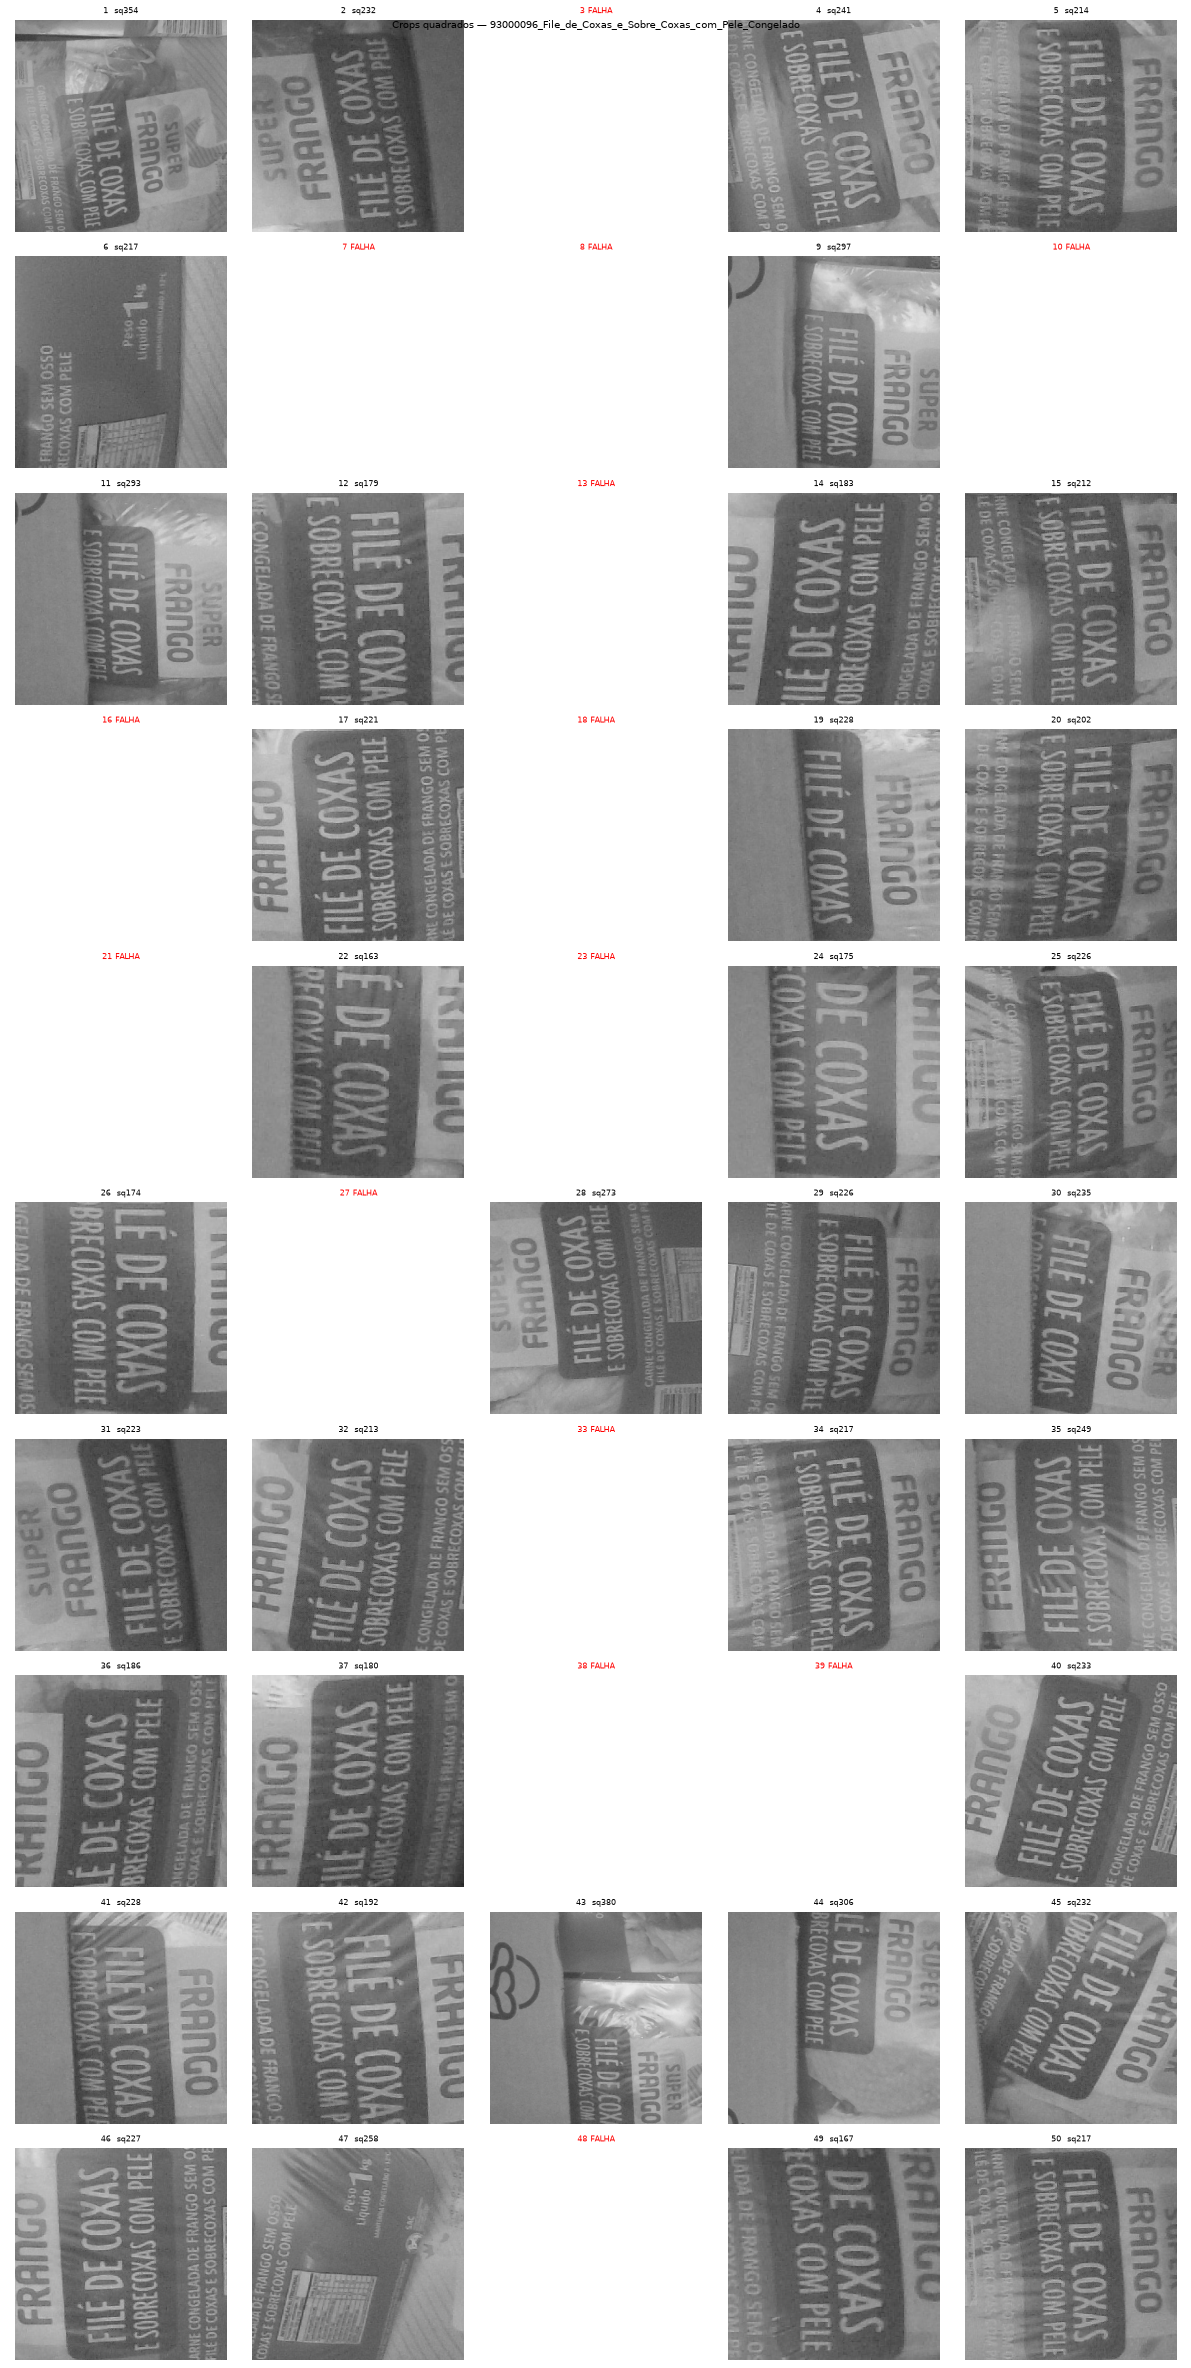
\includegraphics[width=0.85\textwidth]{resultados-exemplo/bandeja/93000096_File_de_Coxas_e_Sobre_Coxas_com_2_crops.png}
\caption{Filé de Coxas e Sobre Coxas com Pele Congelado (bandeja).}
\end{figure}

\begin{figure}[H]
\centering
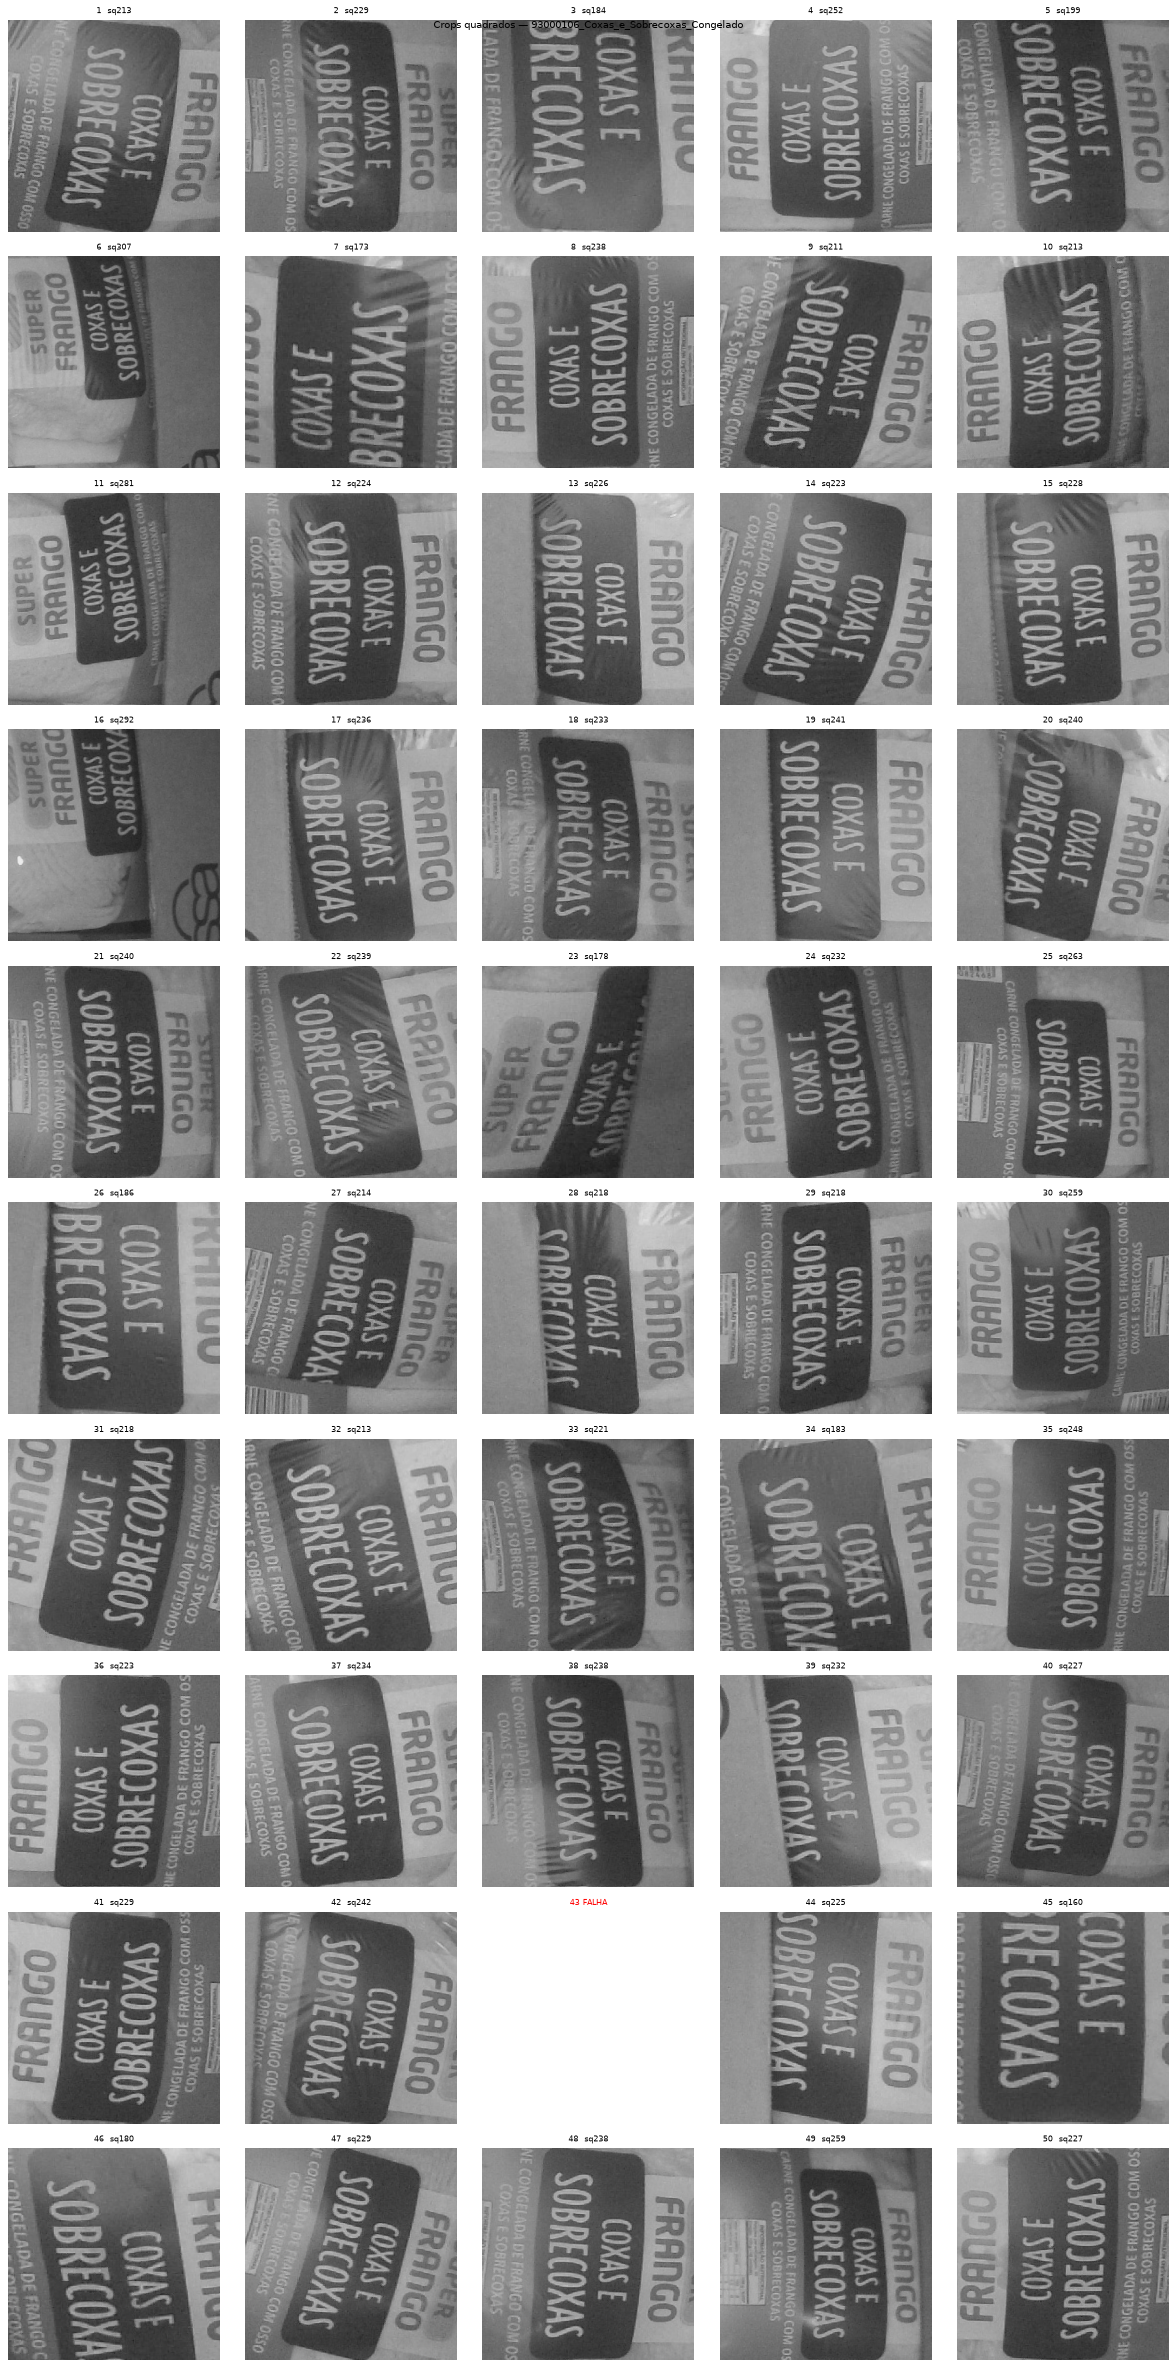
\includegraphics[width=0.85\textwidth]{resultados-exemplo/bandeja/93000106_Coxas_e_Sobrecoxas_Congelado_2_crops.png}
\caption{Coxas e Sobrecoxas Congelado (bandeja).}
\end{figure}

\begin{figure}[H]
\centering
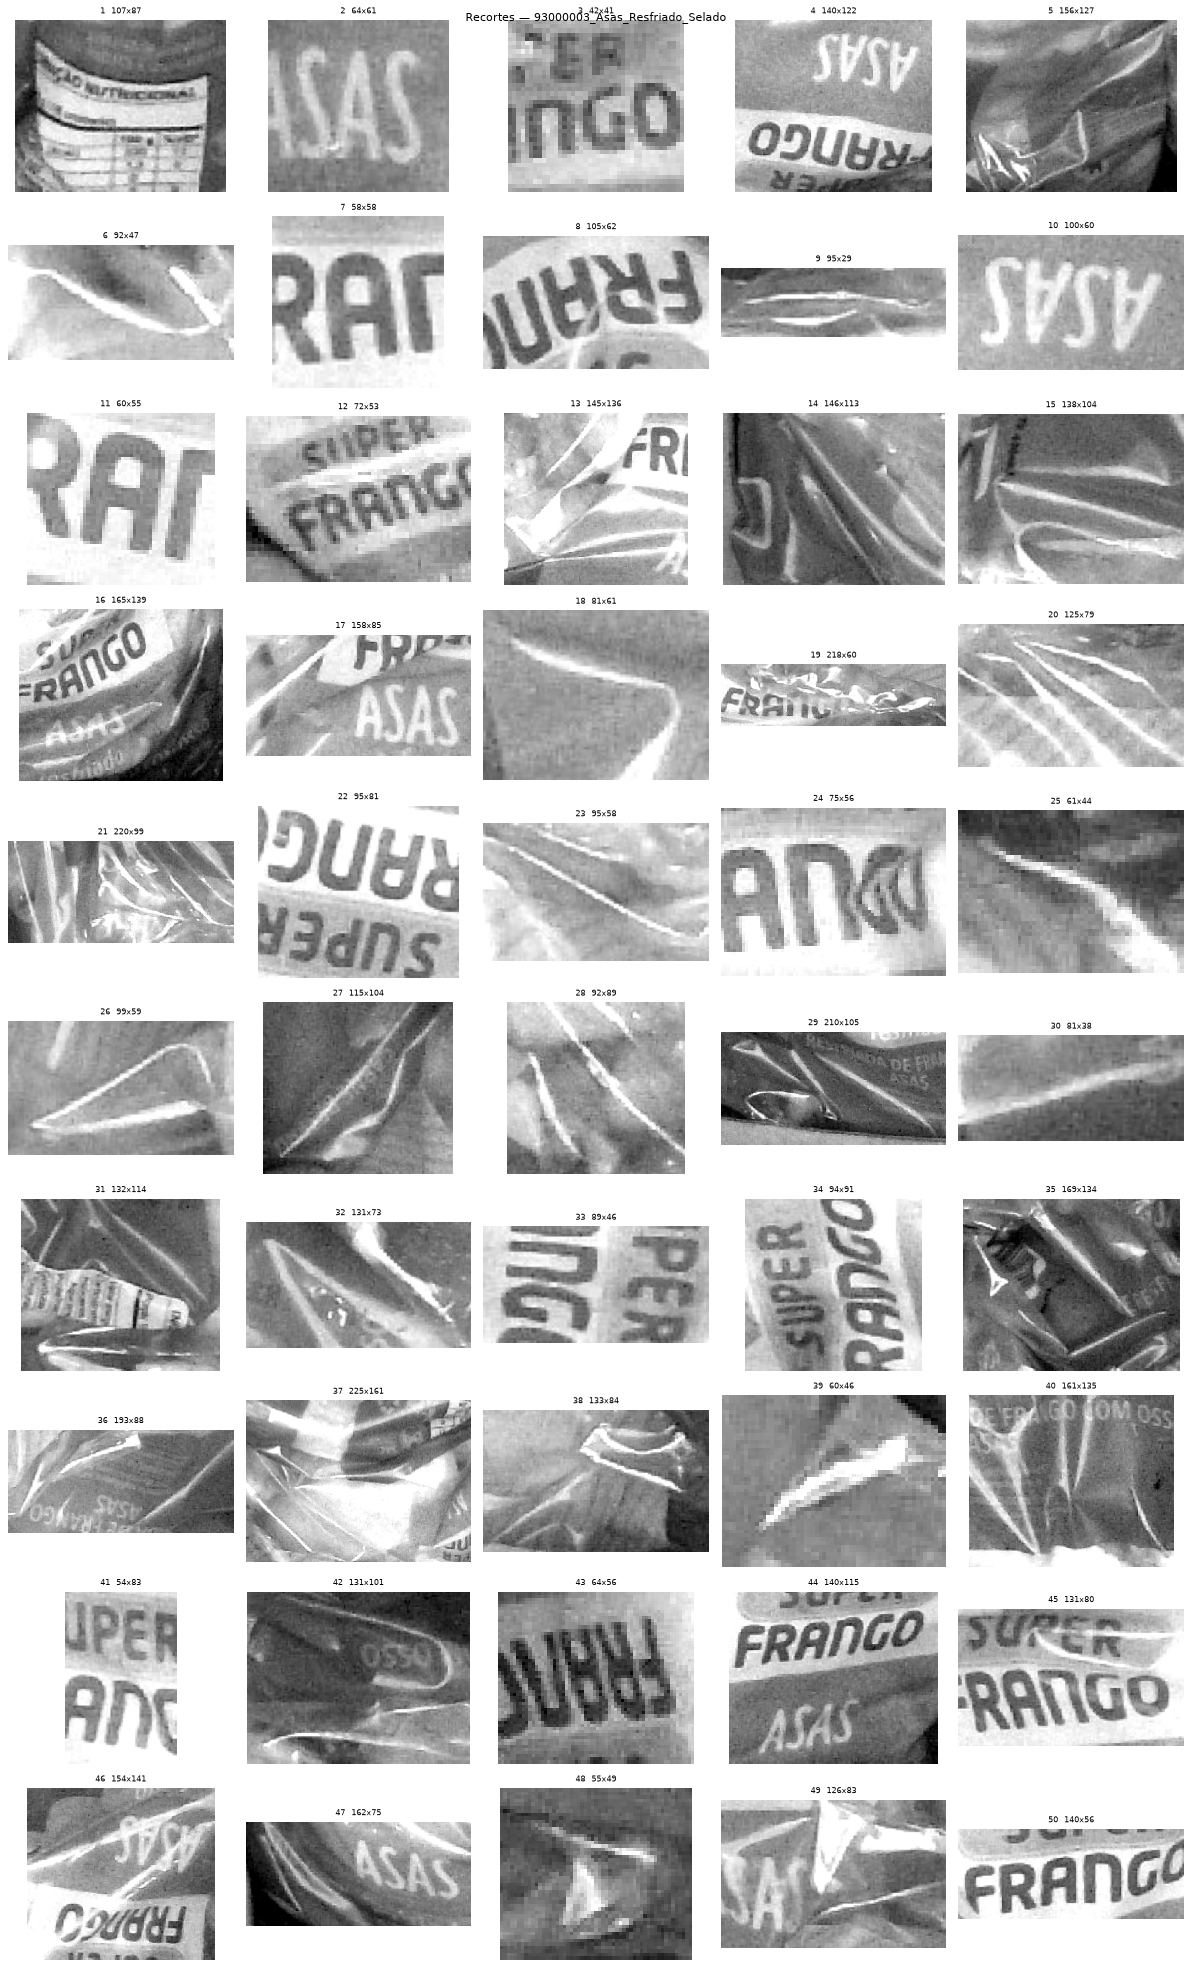
\includegraphics[width=0.85\textwidth]{resultados-exemplo/selado/93000003_Asas_Resfriado_Selado_2_recortes.png}
\caption{Asas Resfriado Selado.}
\end{figure}

\begin{figure}[H]
\centering
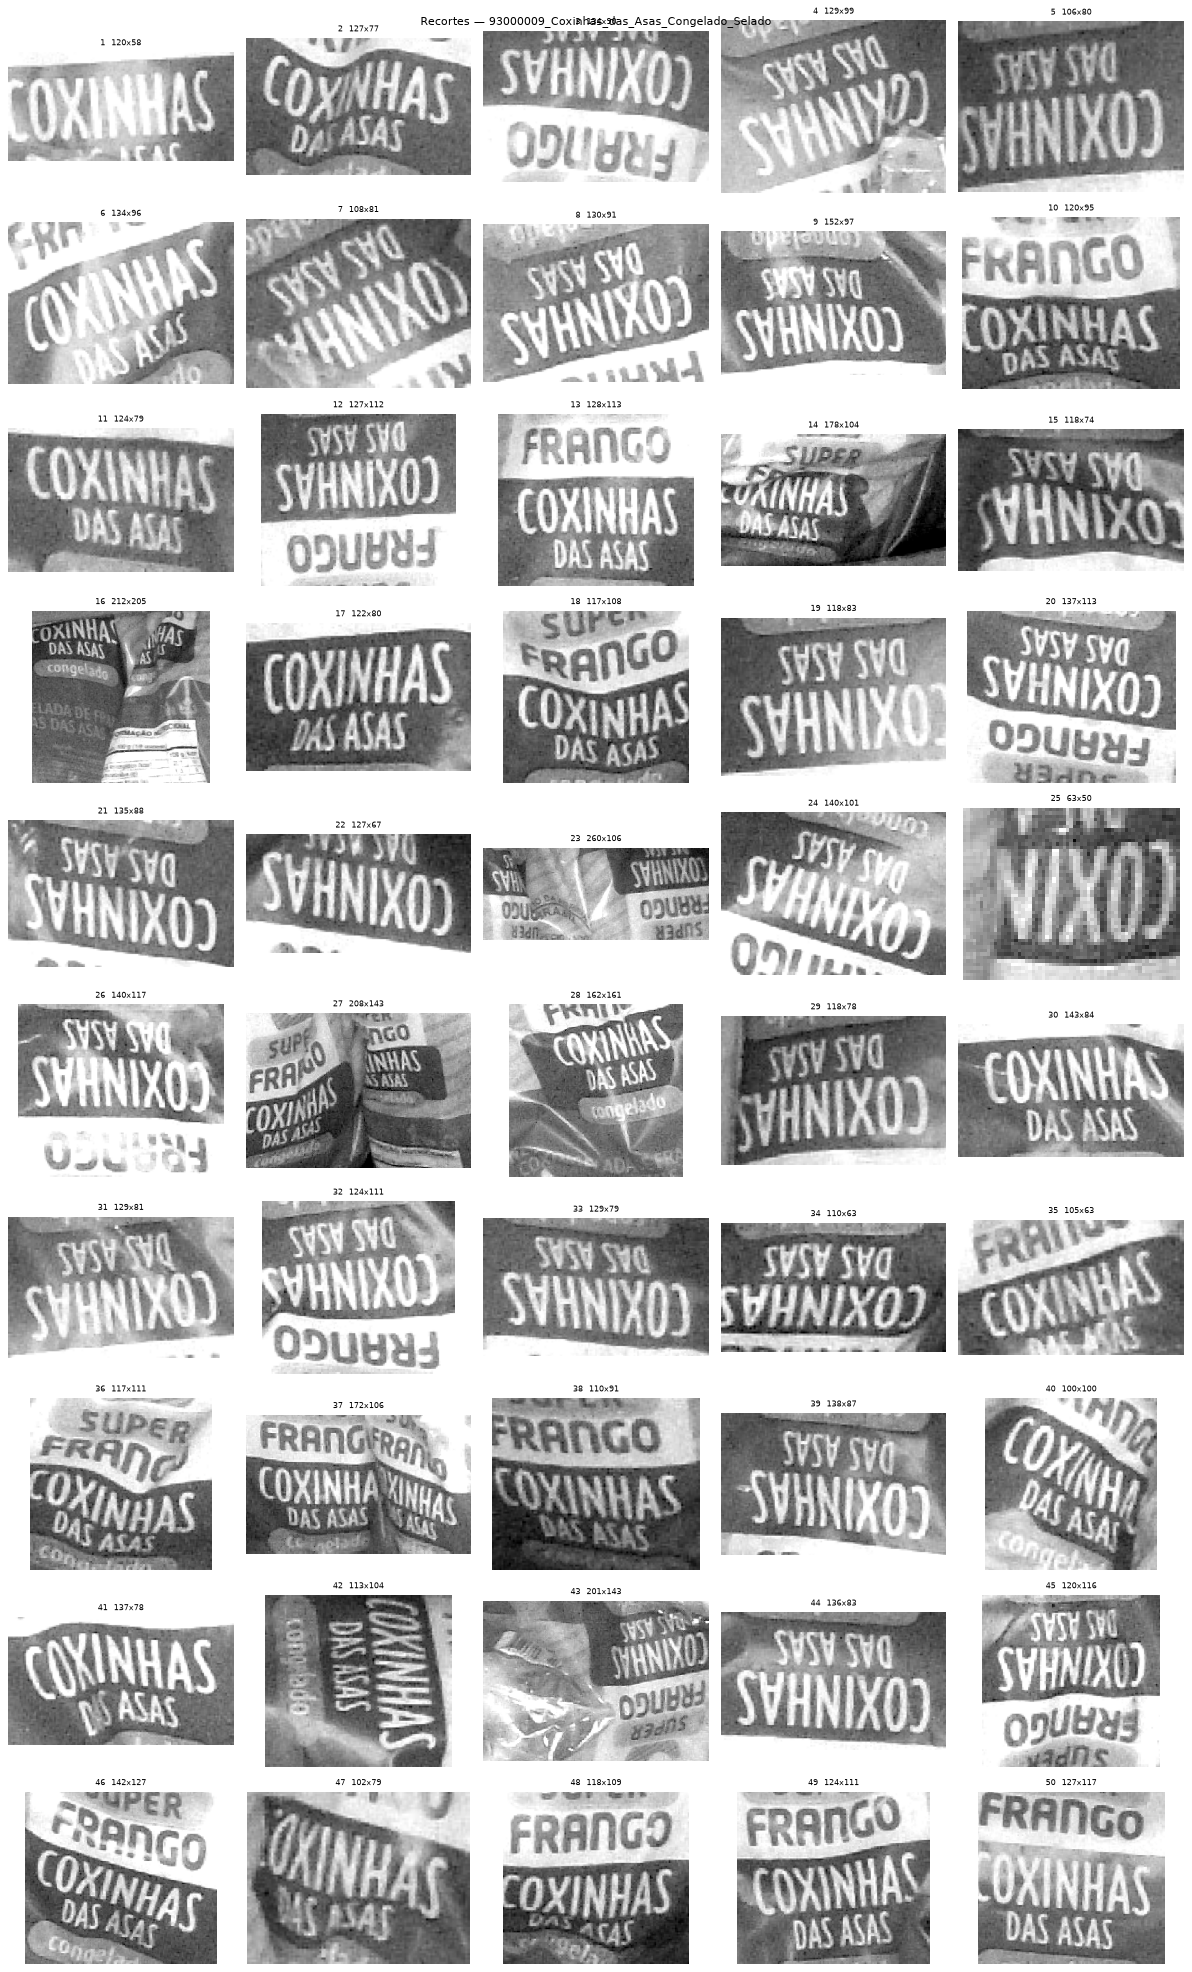
\includegraphics[width=0.85\textwidth]{resultados-exemplo/selado/93000009_Coxinhas_das_Asas_Con_2_recortes.png}
\caption{Coxinhas das Asas Congelado Selado.}
\end{figure}

\begin{figure}[H]
\centering
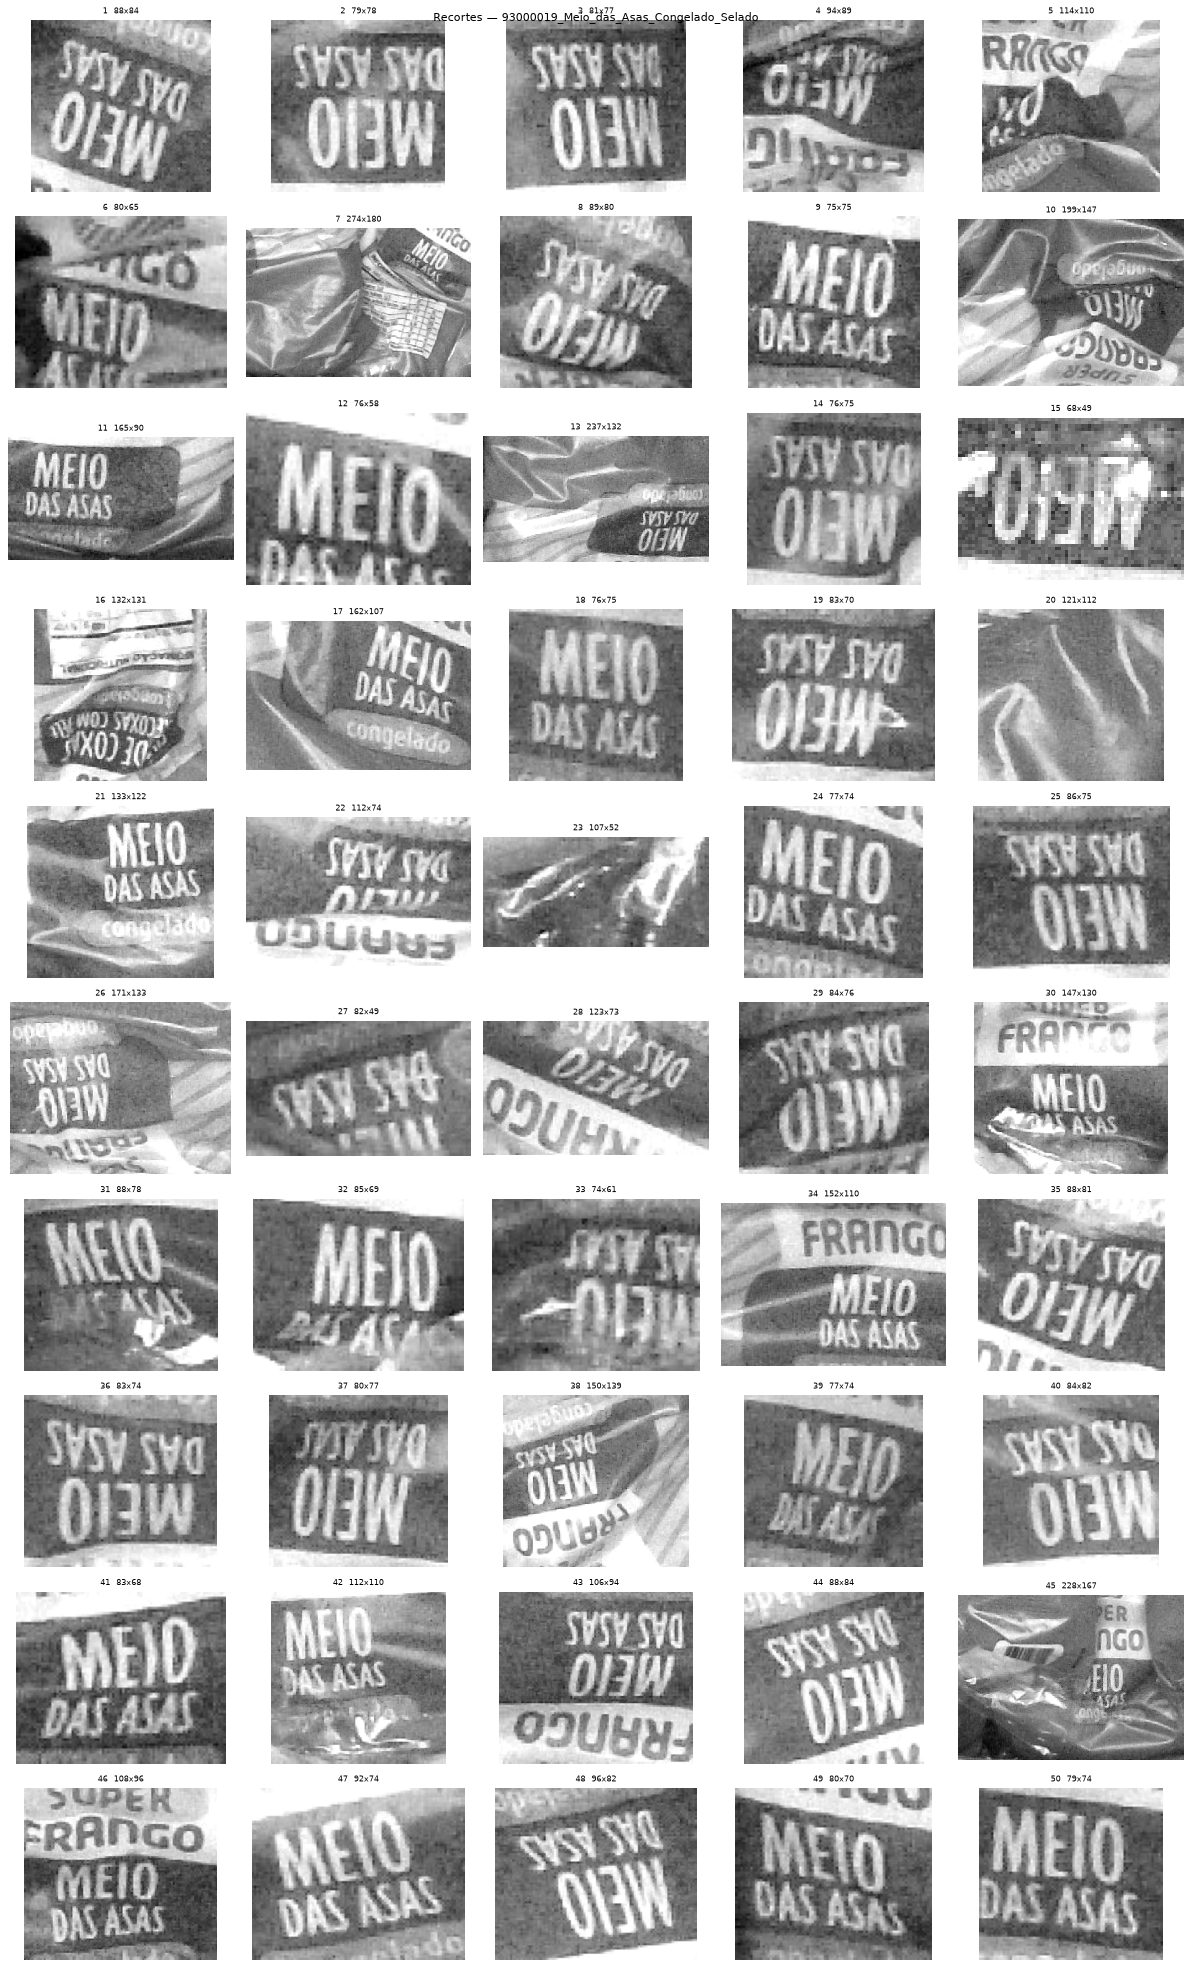
\includegraphics[width=0.85\textwidth]{resultados-exemplo/selado/93000019_Meio_das_Asas_Congela_2_recortes.png}
\caption{Meio das Asas Congelado Selado.}
\end{figure}

\begin{figure}[H]
\centering
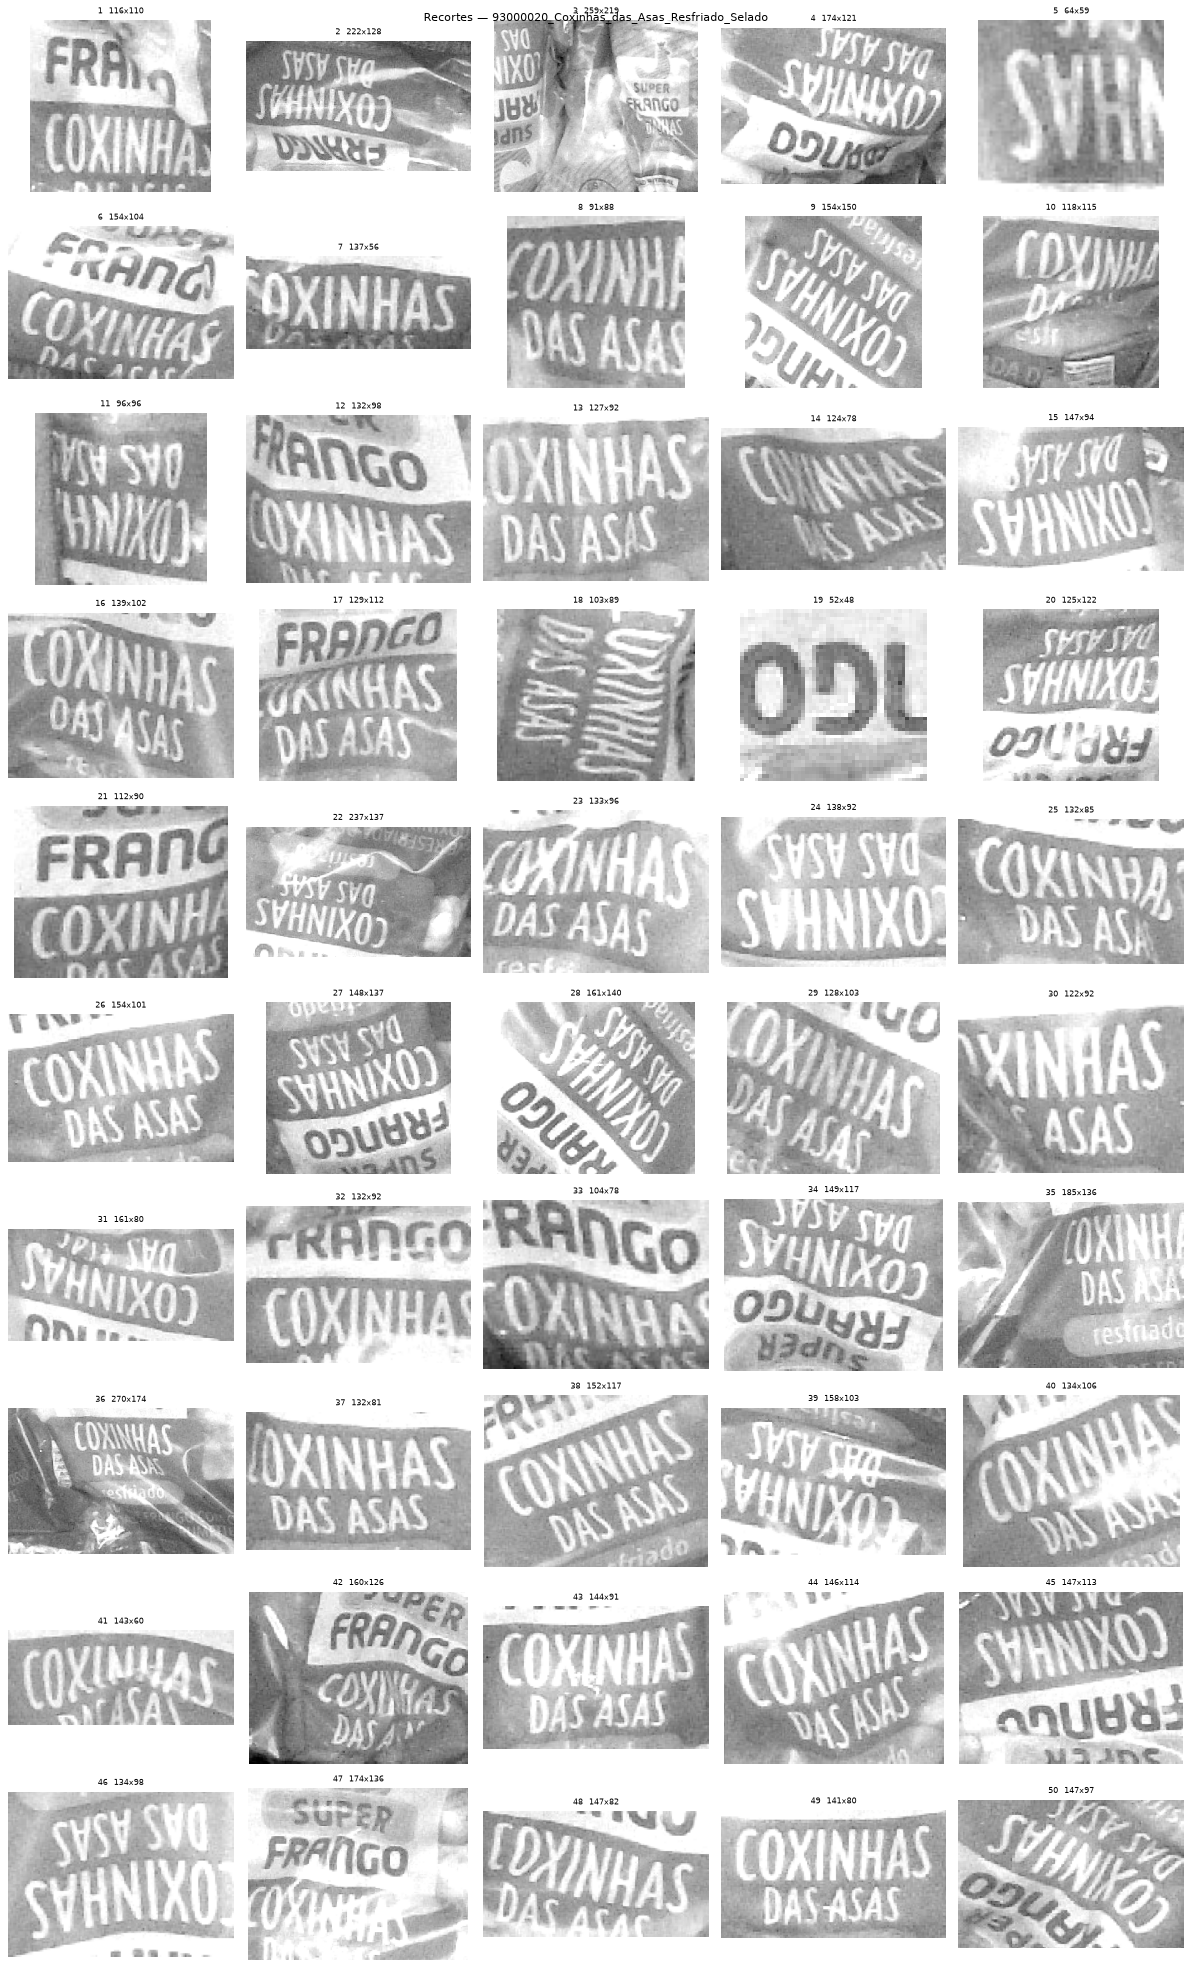
\includegraphics[width=0.85\textwidth]{resultados-exemplo/selado/93000020_Coxinhas_das_Asas_Res_2_recortes.png}
\caption{Coxinhas das Asas Resfriado Selado.}
\end{figure}

\begin{figure}[H]
\centering
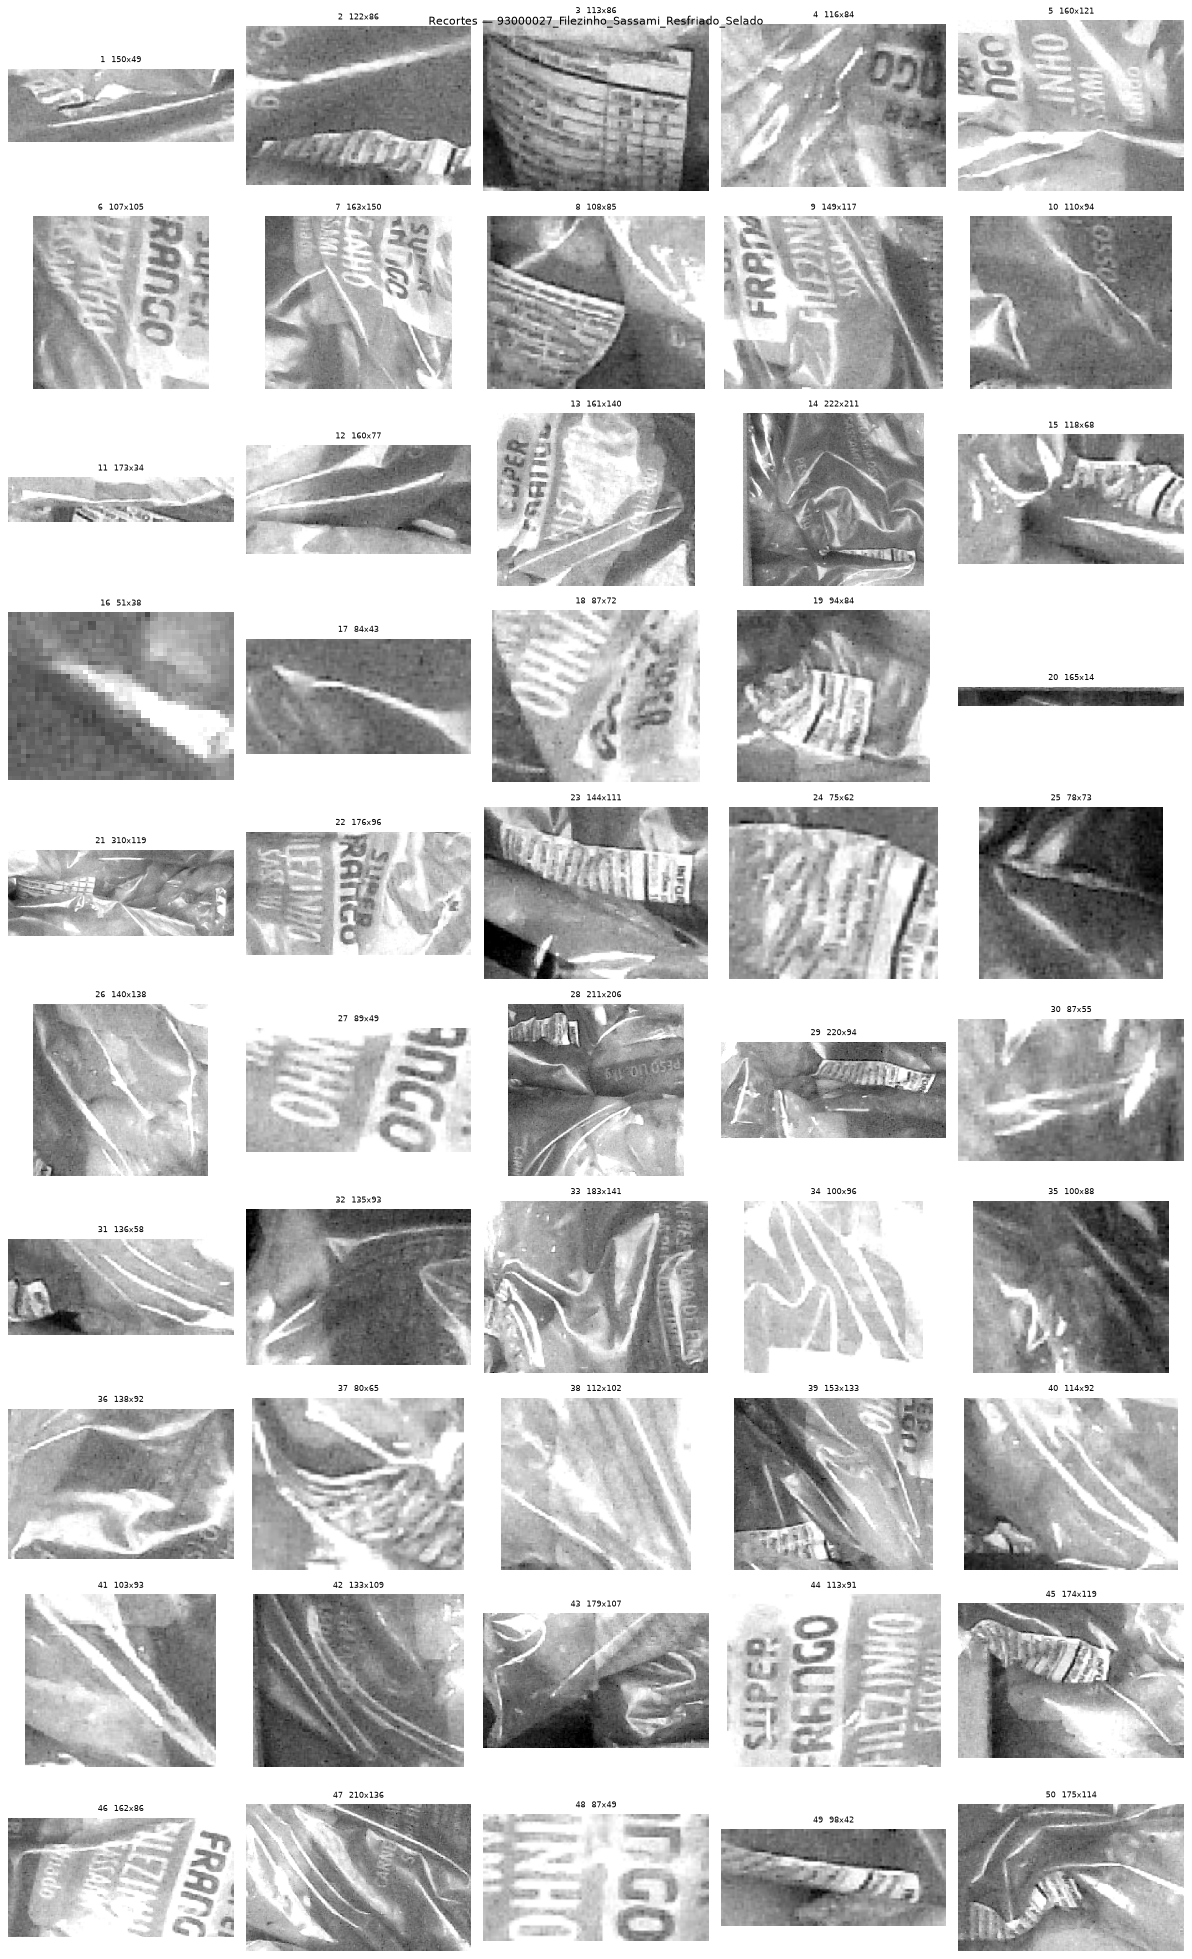
\includegraphics[width=0.85\textwidth]{resultados-exemplo/selado/93000027_Filezinho_Sassami_Res_2_recortes.png}
\caption{Filezinho Sassami Resfriado Selado.}
\end{figure}

\begin{figure}[H]
\centering
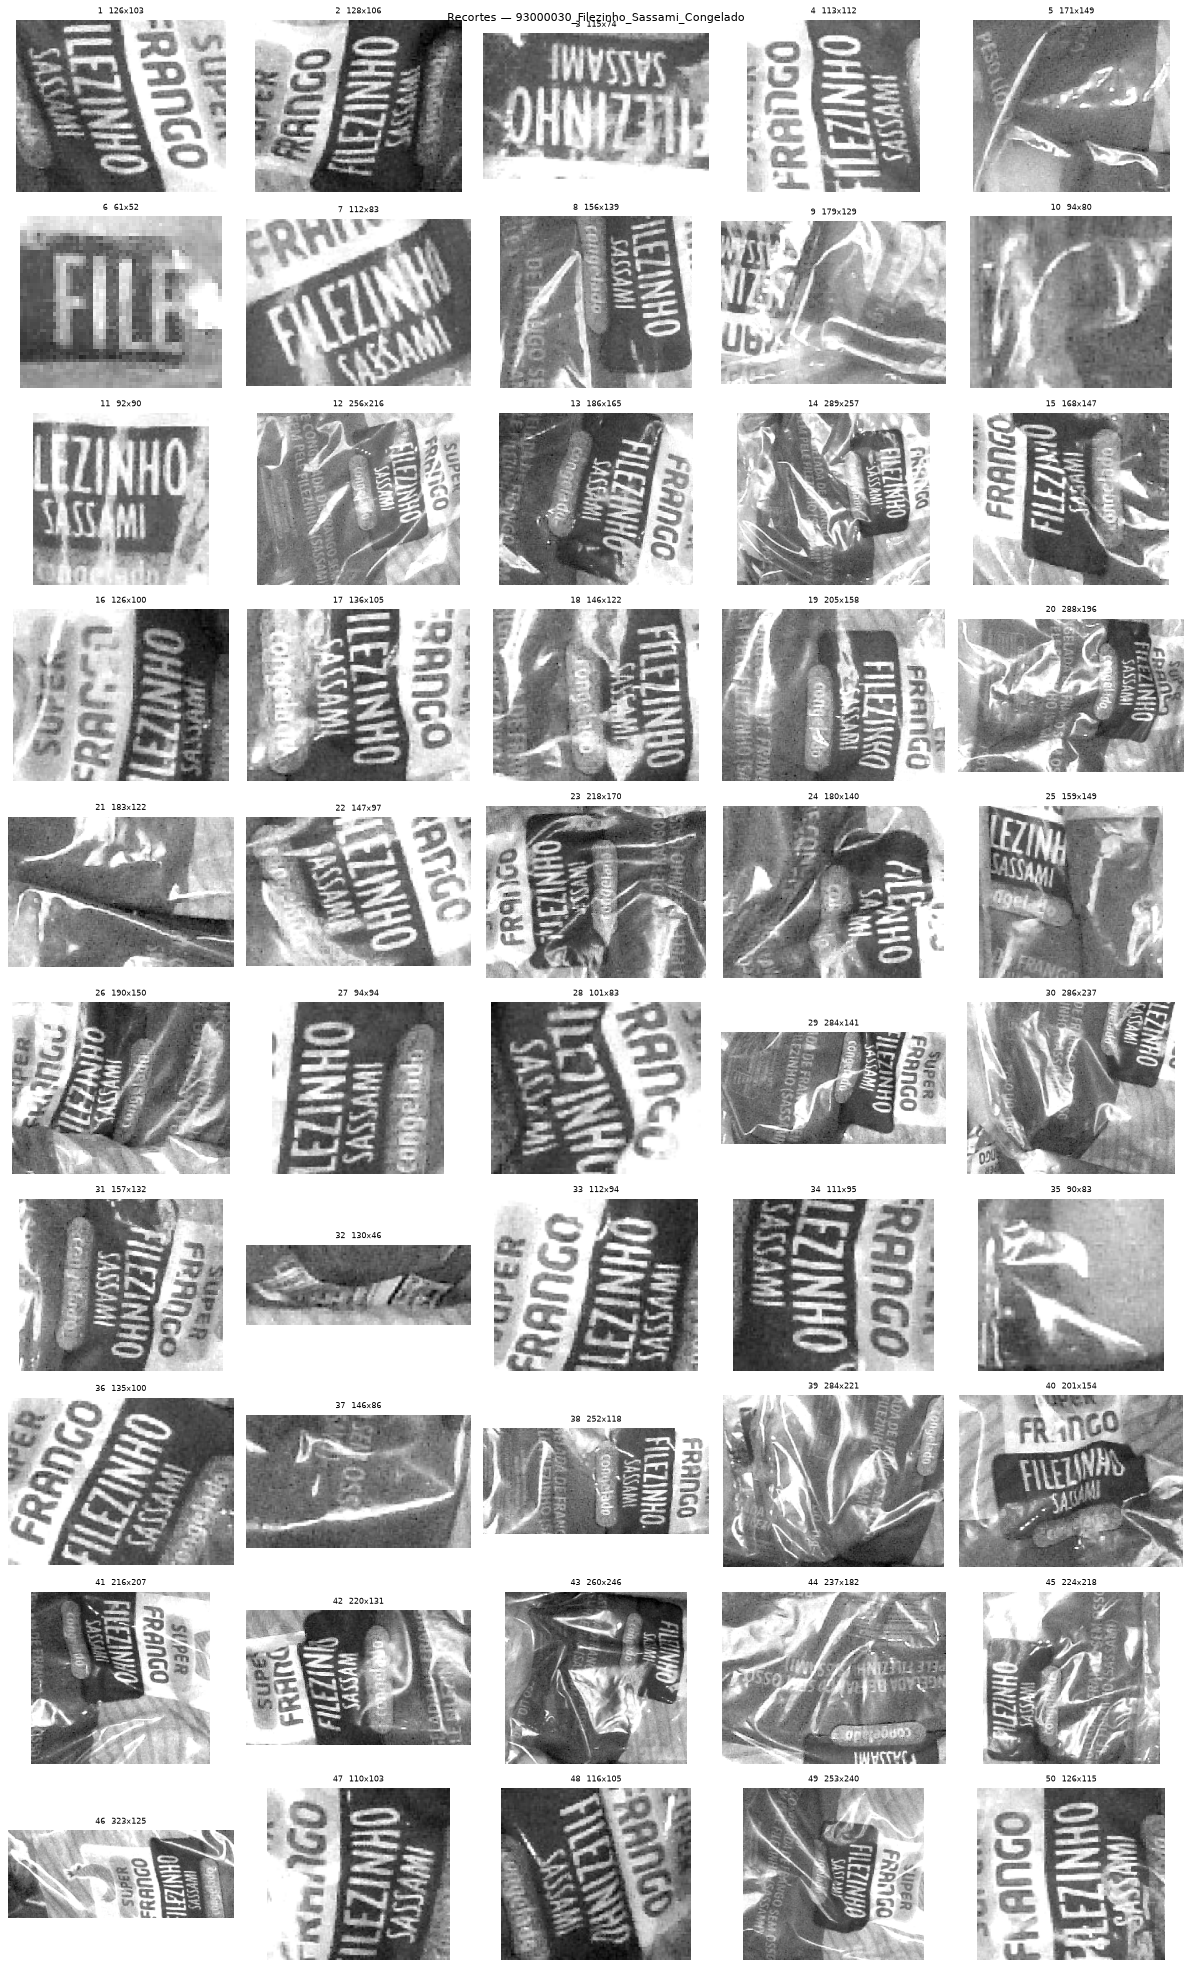
\includegraphics[width=0.85\textwidth]{resultados-exemplo/selado/93000030_Filezinho_Sassami_Con_2_recortes.png}
\caption{Filezinho Sassami Congelado.}
\end{figure}

\begin{figure}[H]
\centering
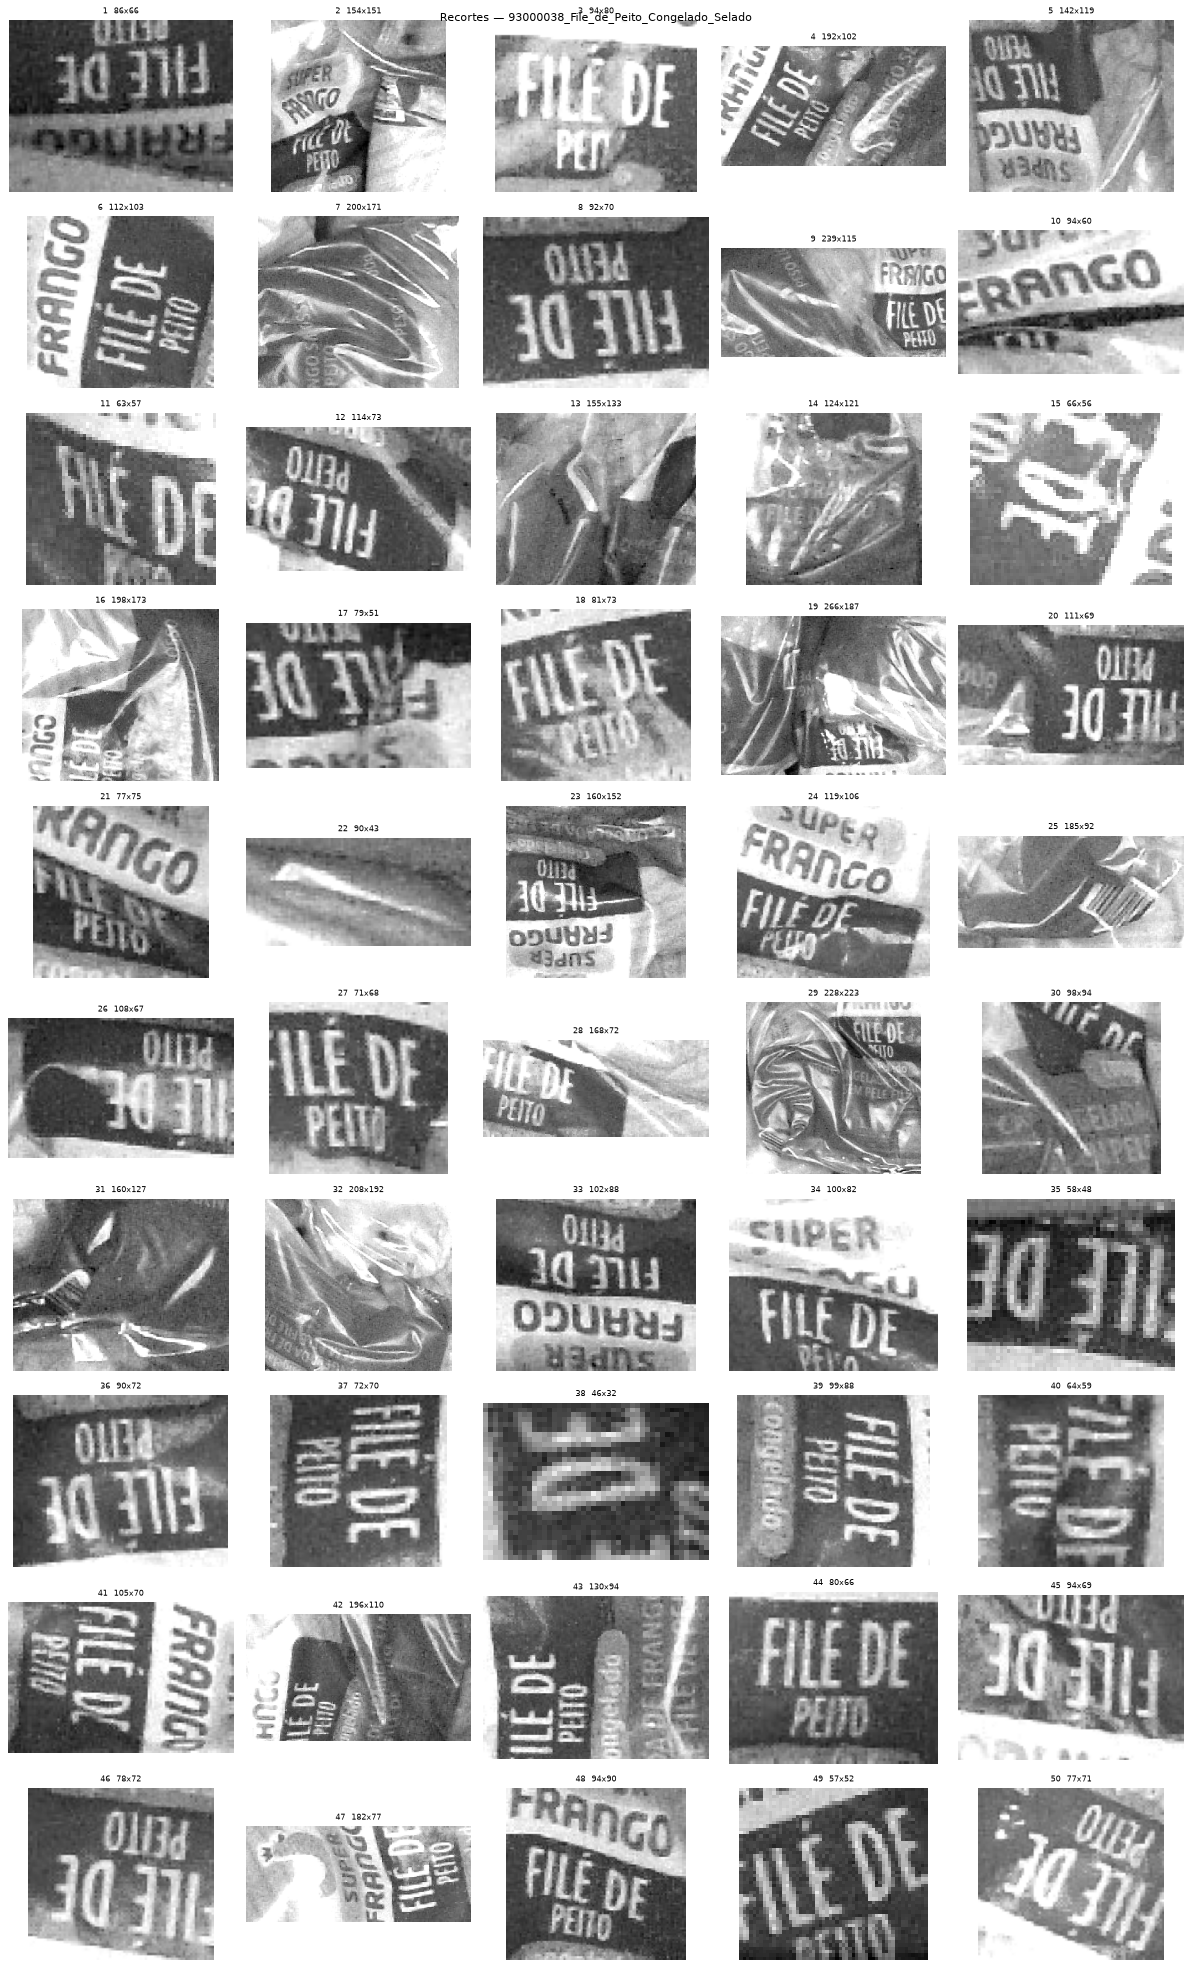
\includegraphics[width=0.85\textwidth]{resultados-exemplo/selado/93000038_File_de_Peito_Congela_2_recortes.png}
\caption{Filé de Peito Congelado Selado.}
\end{figure}

\begin{figure}[H]
\centering
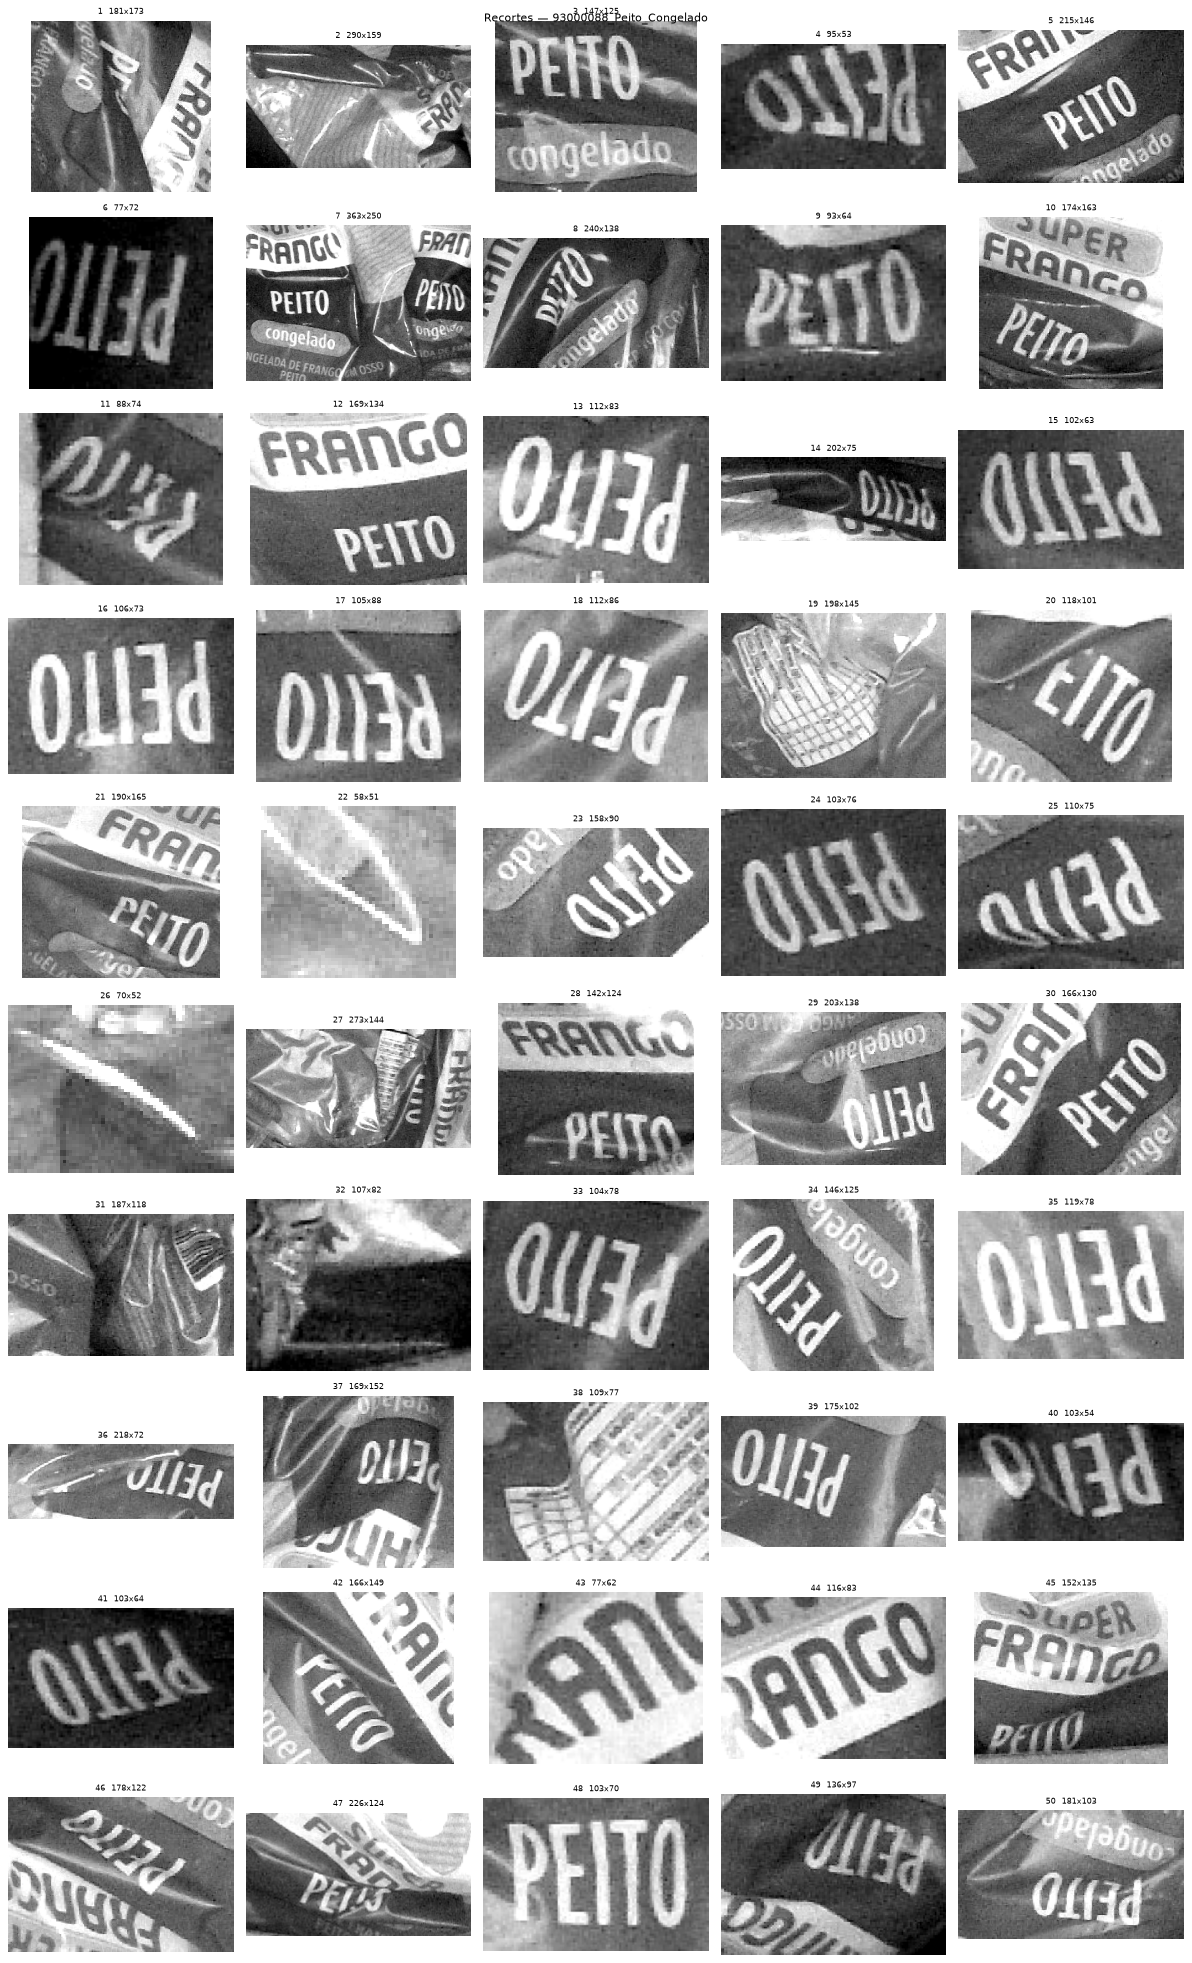
\includegraphics[width=0.85\textwidth]{resultados-exemplo/selado/93000088_Peito_Congelado_2_recortes.png}
\caption{Peito Congelado.}
\end{figure}

\begin{figure}[H]
\centering
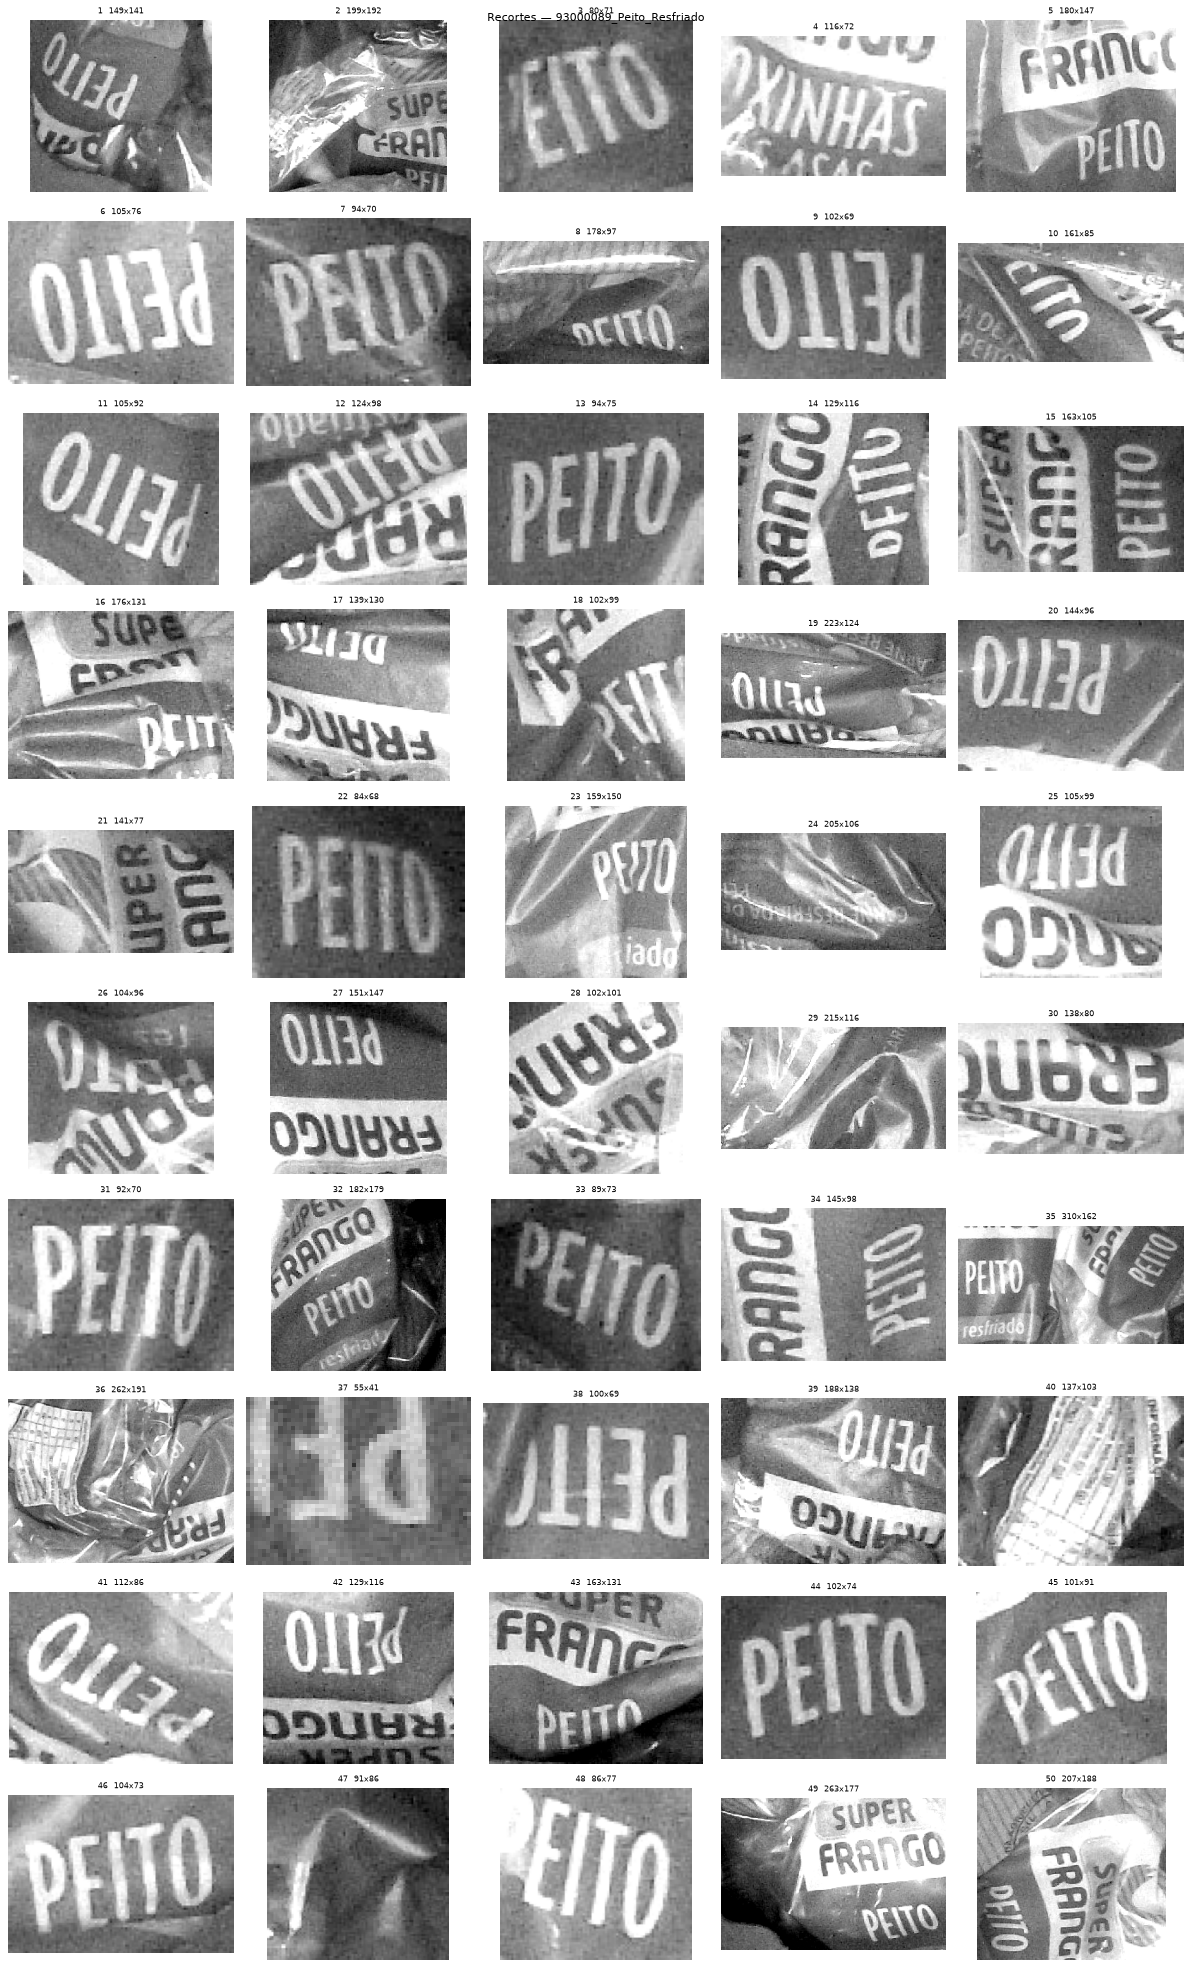
\includegraphics[width=0.85\textwidth]{resultados-exemplo/selado/93000089_Peito_Resfriado_2_recortes.png}
\caption{Peito Resfriado.}
\end{figure}

\begin{figure}[H]
\centering
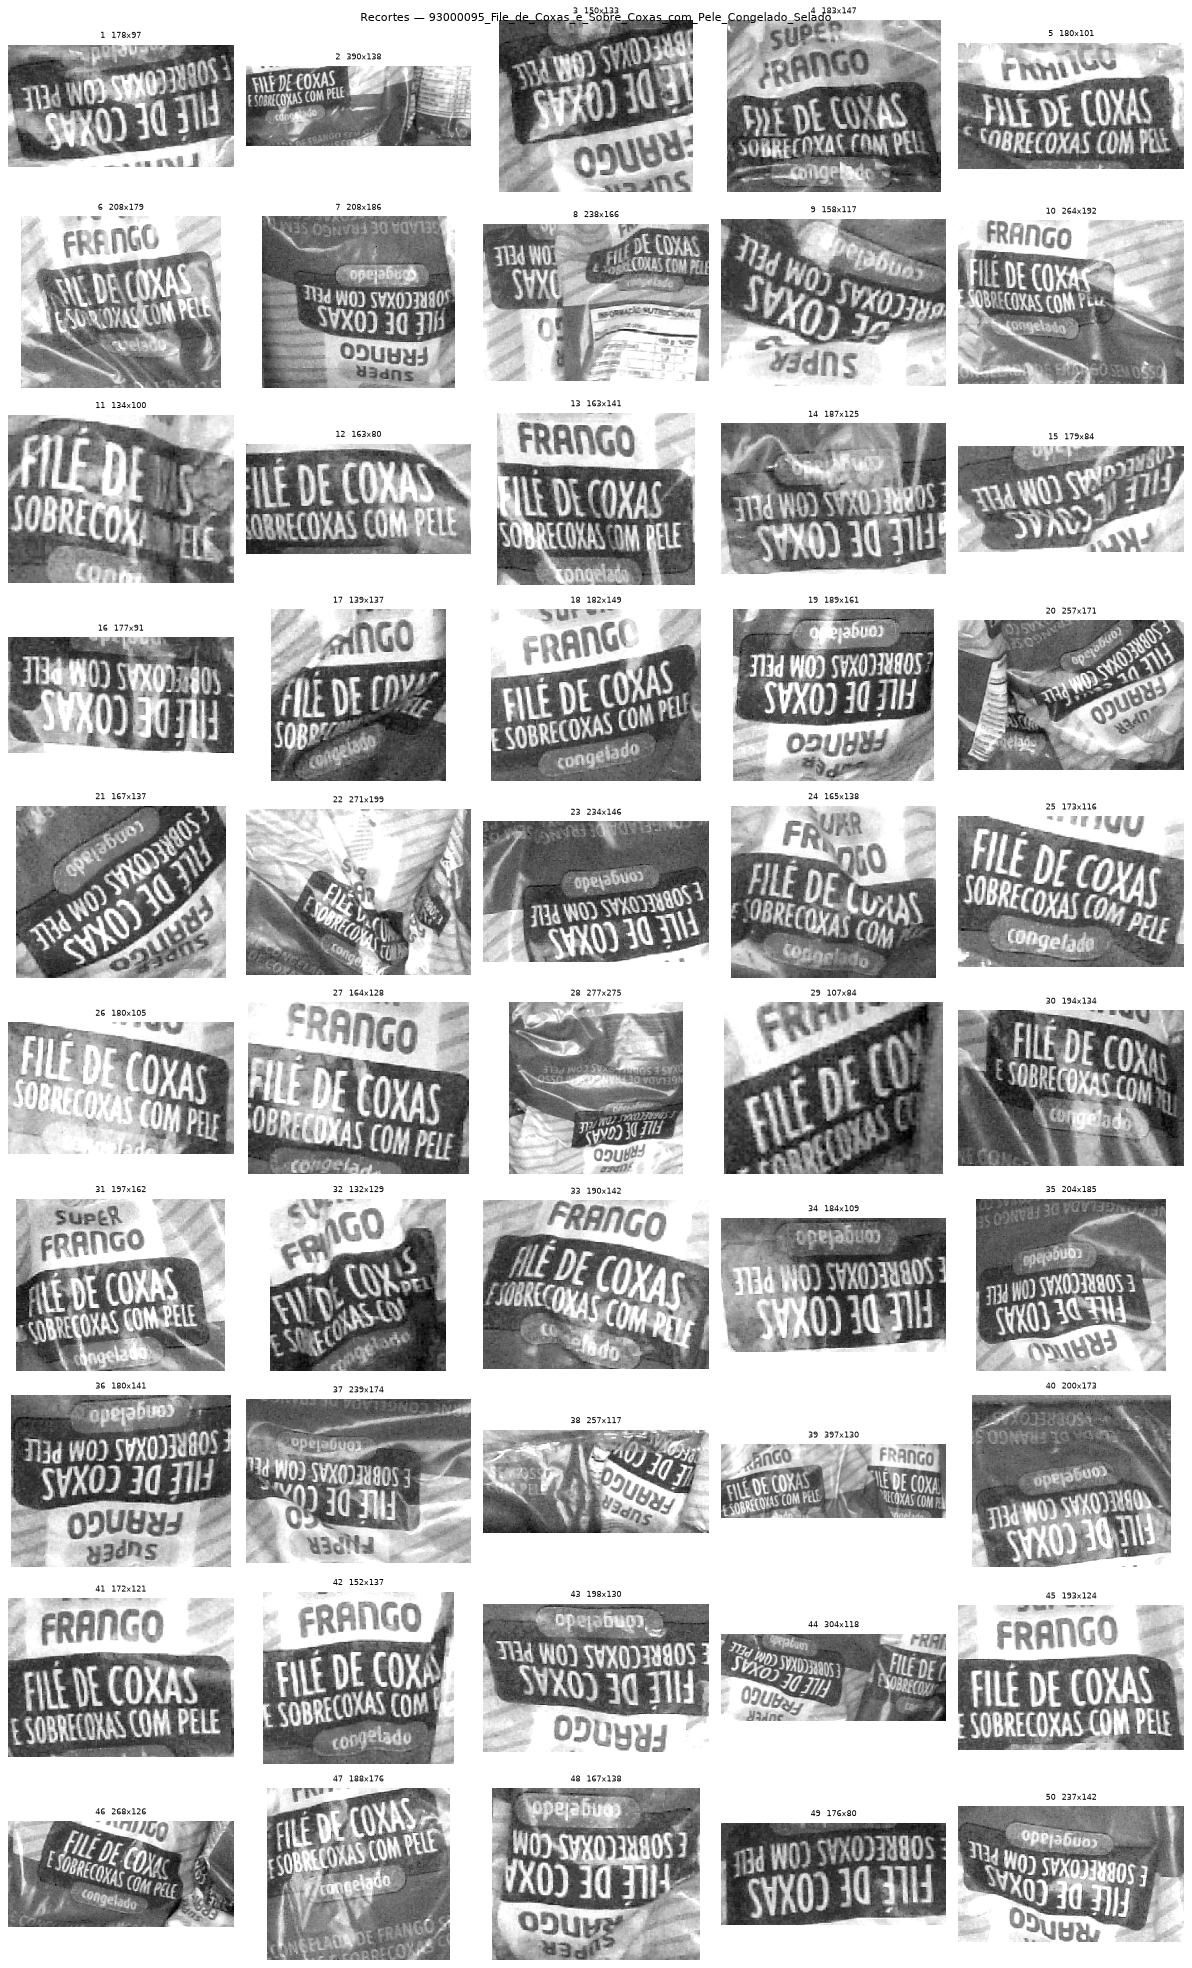
\includegraphics[width=0.85\textwidth]{resultados-exemplo/selado/93000095_File_de_Coxas_e_Sobre_2_recortes.png}
\caption{Filé de Coxas e Sobrecoxas com Pele Congelado Selado.}
\end{figure}

\begin{figure}[H]
\centering
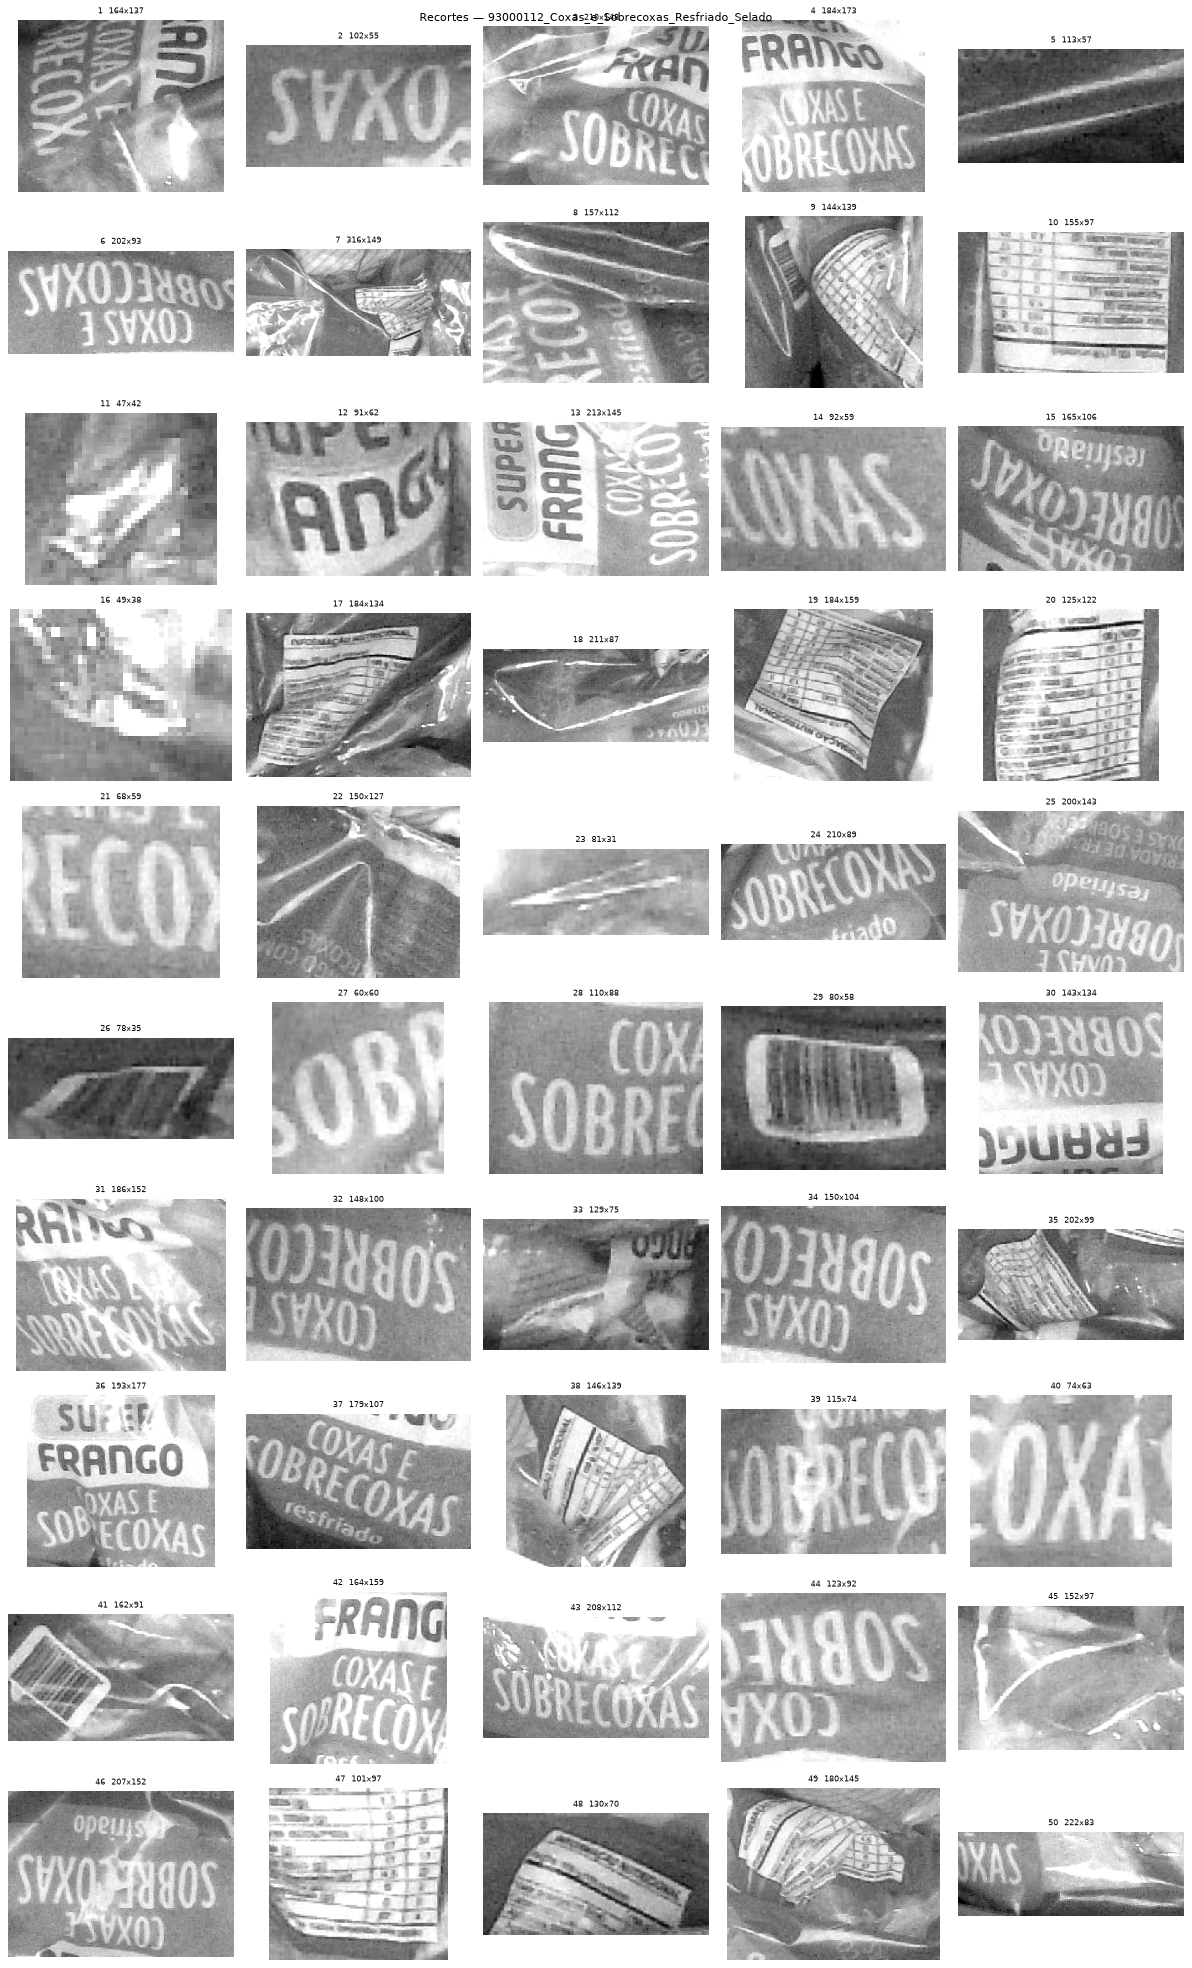
\includegraphics[width=0.85\textwidth]{resultados-exemplo/selado/93000112_Coxas_e_Sobrecoxas_Re_2_recortes.png}
\caption{Coxas e Sobrecoxas Resfriado Selado.}
\end{figure}

\section{Conclusão}

O pipeline de bandeja e o pipeline de selado, apesar de operarem sobre layouts físicos
diferentes, seguem a mesma filosofia de projeto: parâmetros centralizados, etapas
independentes e testáveis isoladamente, e preferência por não gerar recorte a gerar um recorte
errado. Essa escolha de projeto é a mesma adotada na etapa de reconhecimento (T2, ver
\texttt{docs/relatorio-t2.tex}), onde o custo de um falso positivo também é tratado como maior
que o custo de uma detecção perdida.

\section{Direitos autorais}

As imagens do dataset utilizado retratam embalagens e produtos da marca \textbf{Super Frango},
cujos direitos pertencem aos seus respectivos titulares e foram cedidas apenas para uso
acadêmico nesta disciplina. Este relatório e o código associado não fazem nenhuma reivindicação
de direito sobre a marca, o produto ou as imagens originais do dataset.

\end{document}
